%Document Class - Article

\documentclass[14pt]{report}

%Preamble

\title{Universal Interpreter}
\date{10/03/2020}
\author{Jerry Allan Akshay, Shiva Pundir, Rahul R and Sai Kumar}

\usepackage{indentfirst}
\usepackage{array}
\usepackage[utf8]{inputenc}
\usepackage{graphicx}
\usepackage{geometry}
\usepackage{extsizes}
\usepackage{fancyhdr}
\usepackage{titleref}
\usepackage{tabularx}
\usepackage{lmodern} % for bold teletype font
\usepackage{amsmath}  % for \hookrightarrow
\usepackage{xcolor}   % for \textcolor
\usepackage{listings}
\usepackage{subfig}
\usepackage{float}


\lstset{
  basicstyle=\ttfamily,
  columns=fullflexible,
  frame=single,
  breaklines=true,
  postbreak=\mbox{\textcolor{red}{$\hookrightarrow$}\space},
}
\graphicspath{ {./images/} }
\usepackage [english]{babel}
\usepackage [autostyle, english = american]{csquotes}
\MakeOuterQuote{"}

\newcommand{\changefont}{
    \fontsize{10}{10}\selectfont
}

%Page Margins and Dimensions
\geometry{		
	a4paper,
	total={170mm,257mm},
	left=25mm,
	top=25mm,
	right=25mm,
	bottom=25mm,
	}

%Header
\pagestyle{fancy}
\fancyhf{}
\rhead{Universal Interpreter}

\renewcommand{\contentsname}{Table of Contents}

\renewcommand{\headrulewidth}{2pt}
\renewcommand{\footrulewidth}{0.4pt}



\begin{document} %Document Begins

	%Title Page

 	\maketitle
	\pagenumbering{gobble} %Disable Page Numbering

	\newpage

	%Acknowledgement

	\chapter*{Acknowledgement}\label{chapter}
		
		\lhead{\titleref{chapter}}

		The satisfaction and euphoria that accompany the successful completion of any task would be incomplete without the mention of the people who made it possible, whose constant guidance and encouragement crowned our effort with success. \newline
		 
		We express our sincere gratitude to the University Visvesvaraya College of Engineering, Bangalore, for having given us the opportunity to carry out this project. We would also like to thank our Principal, Dr. H. N. Ramesh, for providing us all the facilities to work on this project. \newline
	 
		We wish to place on record our grateful thanks to Dr. Dilip Kumar, Head of the Department, Department of Computer Science and Engineering, for providing us a wonderful opportunity to learn and the needful resources for this project. \newline 
	 
		We consider it a privilege and an honour to express our sincere gratitude to our guide, Mrs. P. Deepa Shenoy, for her valuable guidance throughout the tenure of this project work, and whose support and encouragement made this work possible.  \newline
	 
		We also thank our parents and our friends for their help, encouragement and support. Last but not the least; we thank God Almighty, without whose blessings this wouldn't have been possible. \newline 

		\hfill \textbf{Thanking You} 

		\hfill Jerry Allan Akshay 

		\hfill Shiva Pundir 

		\hfill Rahul R. 

		\hfill Sai Kumar 

	%Abstract

	\chapter*{Abstract}\label{chapter}
		
	\lhead{\titleref{chapter}}

		The project 'Universal Interpreter' was built as an application to help the differently-abled people, i.e. deaf, dumb, blind or combination of any, by using Image Recognition and AI/ML. \newline
		
		The present world we live in, a world dominated by visual and audio peripherals, can prove to be a tough place to live in for differently abled people. Hence, this project was inspired by the need to use the very same dominating technologies to help the differently abled overcome their challenges. \newline 

		With Universal Interpreter, we make use of Morse Codes and the American Sign Language - two of the standardised forms of communication all over the world - to ensure that any differently-abled person can use the application for its intended purposes.\newline 

	

	%Table of Contents

	\lhead{Table of Contents}

	\renewcommand{\footrulewidth}{0pt}

	\tableofcontents

	\newpage

	%List of Figures and Tables

	\listoffigures

	\newpage

	\renewcommand{\footrulewidth}{0.4pt}

	\pagenumbering{arabic} %Use Page Numbering from here


	%Footer
	\fancyfoot[R]{\changefont Page \thepage}

	%Introduction

	\chapter{Introduction}\label{chapter1}
		
	\lhead{\titleref{chapter1}}
	
		% Redefine the plain page style
		\fancypagestyle{plain}{%
		\fancyhf{}%
		\fancyfoot[R]{Page \thepage}%
		\renewcommand{\headrulewidth}{0pt}% Line at the header invisible
		\renewcommand{\footrulewidth}{0.4pt}% Line at the footer visible
		}

		\section{Problem Definition}
			The world we live in is a world dominated by technology made for people with no impairments. Smartphones and Computers form a major portion of this technology. In the current age and time, most of the communication between people takes place through the use of smartphones and computers via SMS(s), Emails WhatsApp messages and so forth. \\
			
			As such, physically impaired people don't get to reap the benefits of smartphones, computers and other technologies catered to the non-impaired as there are no appropriate interfaces designed for use by them on these devices.
		
			\section{Objectives}
			The main objective of this project is to set up interfacing mechanisms for the physically-impaired - specifically the deaf, dumb and blind - and design an application for the purpose of communication between the users of the aforementioned application. The objectives can be postulated as follows:
			\begin{itemize}
				\item To set up interfacing mechanisms using Morse Codes, Text, Speech and the American Sign Language. 
				\item To design an Android Application for the purposes of communication using the aformentioned interfaces.
				\item To structure and use a no-SQL database in the appropriate format for the purpose of use of the Android Application.
				\item To train and use a Neural Network Model for the purposes of recognizing the Hand Gestures in the form of the American Sign Language through the use of a Camera.
			\end{itemize}
				\section{Standardised Forms of Communication}
				In general, communication is simply the act of transferring information from one place, person or group to another. Every communication involves (at least) one sender, a message and a recipient. This may sound simple, but communication is actually a very complex subject. The transmission of the message from sender to recipient can be affected by a huge range of things. These include our emotions, the cultural situation, the medium used to communicate, and even our location. The complexity is why good communication skills are considered so desirable by employers around the world: accurate, effective and unambiguous communication is actually extremely hard.\\

				With regards to communication, there are various internationally accepted and standardised forms of communication. These standardised forms imply the universal understanding of the information being conveyed with the help of the standardised medium.\\

				Since our project is aimed to help the physically impaired such as those who are deaf, dumb, blind, or a combination of these, we make use of two particular standardised forms of communication that are proven to be used effectively for communication by the physically impaired, namely Morse Codes and the American Sign Language (ASL). These two forms of communication are discussed in detail below. 
			\subsection{Morse Codes}

				\begin{figure}[h]
					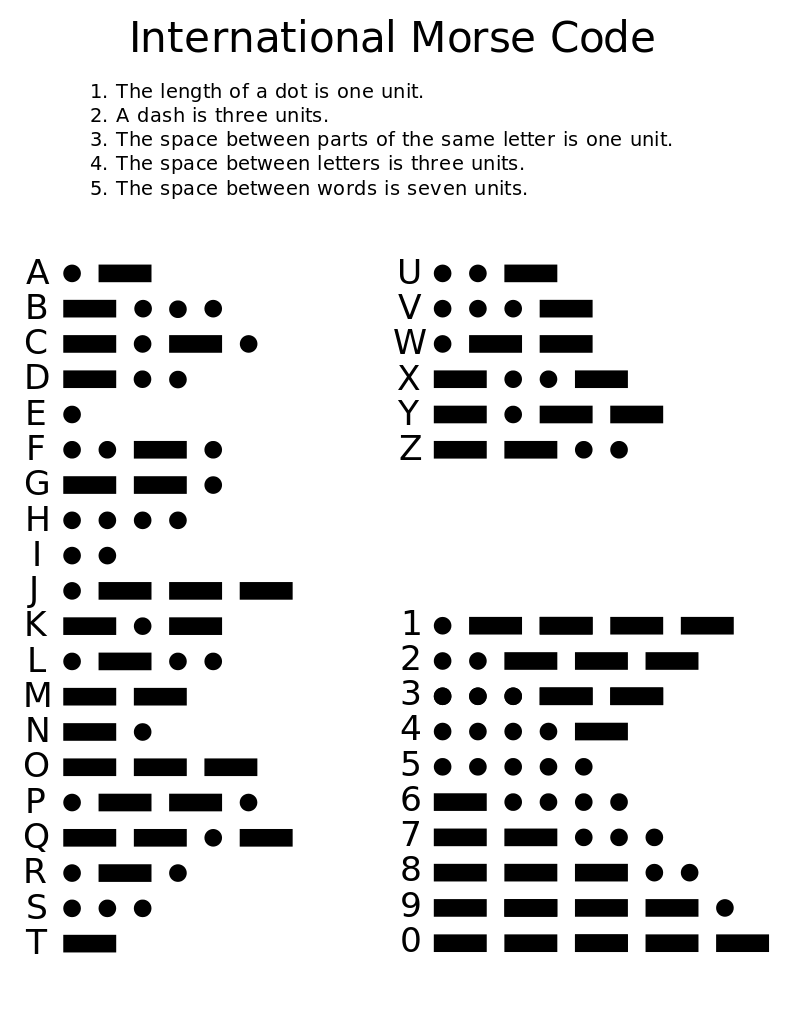
\includegraphics[width=12cm]{Morse Code.png}
					\centering
					\caption{The International Morse Code}
				\end{figure}

				Morse code is a method used in telecommunication to encode text characters as standardized sequences of two different signal durations, called dots and dashes or dits and dahs. Morse code is named for Samuel Morse, an inventor of the telegraph.\\

				The International Morse Code encodes the 26 English letters A through Z, some non-English letters, the Arabic numerals 0 through 9 and a small set of punctuation and procedural signals (prosigns). There is no distinction between upper and lower case letters. Each Morse code symbol is formed by a sequence of dots and dashes. The dot duration is the basic unit of time measurement in Morse code transmission. The duration of a dash is three times the duration of a dot. Each dot or dash within a character is followed by a period of signal absence, called a space, equal to the dot duration. The letters of a word are separated by a space of duration equal to three dots, and the words are separated by a space equal to seven dots. To increase the efficiency of encoding, Morse code was designed so that the length of each symbol is approximately inverse to the frequency of occurrence in text of the English language character that it represents. Thus the most common letter in English, the letter "E", has the shortest code: a single dot. Because the Morse code elements are specified by proportion rather than specific time durations, the code is usually transmitted at the highest rate that the receiver is capable of decoding. The Morse code transmission rate (speed) is specified in groups per minute, commonly referred to as words per minute.\\
				
				Morse code is usually transmitted by on-off keying of an information-carrying medium such as electric current, radio waves, visible light, or sound waves. The current or wave is present during the time period of the dot or dash and absent during the time between dots and dashes. Morse code can be memorized, and Morse code signalling in a form perceptible to the human senses, such as sound waves or visible light, can be directly interpreted by persons trained in the skill.\\

				Because many non-English natural languages use other than the 26 Roman letters, Morse alphabets have been developed for those languages.\\

				\subsubsection{Applications for the General Public}

					\begin{figure}[h]
						
\includegraphics[width=7cm]{SOS - Morse.png}
						\centering
						\caption{Representation of the SOS Morse Code}
					\end{figure}

					An important application is signalling for help through SOS, "\textbf{. . . \_ \_ \_ . . .}". This can be sent many ways: keying a radio on and off, flashing a mirror, toggling a flashlight, and similar methods. SOS is not three separate characters, rather, it is a prosign SOS, and is keyed without gaps between characters.\\
					
					Some Nokia mobile phones offer an option to alert the user of an incoming text message with the Morse tone "\textbf{. . . \_ \_ . . .}" (representing SMS or Short Message Service). In addition, applications are now available for mobile phones that enable short messages to be input in Morse Code.
				
					\subsubsection{Morse Code as an Assistive Technology}
						Morse code has been employed as an assistive technology, helping people with a variety of disabilities to communicate. For example, the Android operating system versions 5.0 and higher allow users to input text using Morse Code as an alternative to a keypad or handwriting recognition.\\

						Morse can be sent by persons with severe motion disabilities, as long as they have some minimal motor control. An original solution to the problem that caretakers have to learn to decode has been an electronic typewriter with the codes written on the keys. Codes were sung by users; see the voice typewriter employing morse or votem, Newell and Nabarro, 1968.\\

						Morse code can also be translated by computer and used in a speaking communication aid. In some cases, this means alternately blowing into and sucking on a plastic tube ("sip\-and\-puff" interface). An important advantage of Morse code over row column scanning is that once learned, it does not require looking at a display. Also, it appears faster than scanning.\\

						In one case reported in the radio amateur magazine \textit{QST}, an old shipboard radio operator who had a stroke and lost the ability to speak or write could communicate with his physician (a radio amateur) by blinking his eyes in Morse. Two examples of communication in intensive care units were also published in \textit{QST}, Another example occurred in 1966 when prisoner of war Jeremiah Denton, brought on television by his North Vietnamese captors, Morse-blinked the word \textit{TORTURE}. In these two cases, interpreters were available to understand those series of eye-blinks.
					
			\subsection{American Sign Language}
				The American Sign Language (ASL) is a natural language i.e., a natural language or ordinary language is any language that has evolved naturally in humans through use and repetition without conscious planning or premeditation, that serves as the predominant sign language of Deaf communities in the United States and most of Anglophone Canada. Besides North America, dialects of ASL and ASL-based creoles are used in many countries around the world, including much of West Africa and parts of Southeast Asia. ASL is also widely learned as a second language, serving as a lingua franca. ASL is most closely related to French Sign Language (LSF). It has been proposed that ASL is a creole language of LSF, although ASL shows features atypical of creole languages, such as agglutinative morphology.\\

				ASL originated in the early 19th century in the American School for the Deaf (ASD) in West Hartford, Connecticut, from a situation of language contact. Since then, ASL use has propagated widely by schools for the deaf and Deaf community organizations. Despite its wide use, no accurate count of ASL users has been taken. Reliable estimates for American ASL users range from 250,000 to 500,000 persons, including a number of children of deaf adults. ASL users face stigma due to beliefs in the superiority of oral language to sign language.\\

				ASL signs have a number of phonemic components, such as movement of the face, the torso, and the hands. ASL is not a form of pantomime although iconicity plays a larger role in ASL than in spoken languages. English loan words are often borrowed through fingerspelling, although ASL grammar is unrelated to that of English. ASL has verbal agreement and aspectual marking and has a productive system of forming agglutinative classifiers. Many linguists believe ASL to be a subject–verb–object (SVO) language. However, there are several alternative proposals to account for ASL word order.
			
				\begin{figure}[h]
					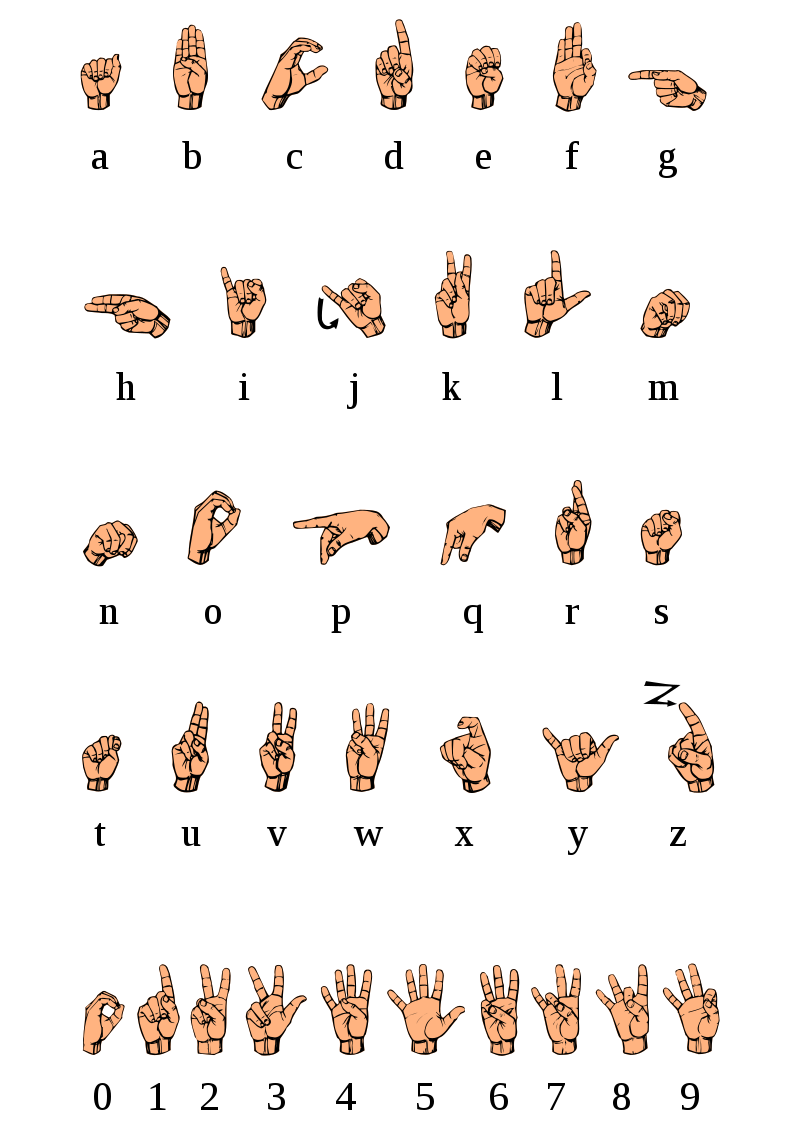
\includegraphics[width=12cm]{ASL Signs.png}
					\centering
					\caption{ASL Hand Signs}
					\label{fig:ASLHandSign}
				\end{figure}

				\subsubsection{Finger-Spelling}
					ASL possesses a set of 26 signs known as the American manual alphabet, which can be used to spell out words from the English language. Such signs make use of the 19 handshapes of ASL.  example, the signs for `p' and `k' use the same handshape but different orientations. A common misconception is that ASL consists only of fingerspelling; although such a method (Rochester Method) has been used, it is not ASL.\\

					Fingerspelling is a form of borrowing, a linguistic process wherein words from one language are incorporated into another. In ASL, fingerspelling is used for proper nouns and for technical terms with no native ASL equivalent. There are also some other loan words which are fingerspelled, either very short English words or abbreviations of longer English words, e.g. O-N from English `on', and A-P-T from English `apartment'. Fingerspelling may also be used to emphasize a word that would normally be signed otherwise.\\
				
		\section{Tools}
			There are various tools that have been used to realize the project Universal Interpreter. The combinatorial usage of these tools has helped to fabricate this project. As such, there are two categories of tools - The Front-end Tools and the Back-end Tools. \\
			
			Front-end and Back-end are terms used by programmers and computer professionals to describe the layers that make up hardware, a computer program or a website which are delineated based on how accessible they are to a user. These two categories of tools are further discussed below. 
			\subsection{Front-end Tools}
				The layer above the back end is the front end and it includes all software or hardware that is part of a user interface. Human or digital users interact directly with various aspects of the front end of a program, including user-entered data, buttons, programs, websites and other features. Most of these features are designed by user experience (UX) professionals to be accessible, pleasant and easy to use. The Front-end tools used for this project are mentioned below.
				\subsubsection{Android Studio}
				Android Studio is the official integrated development environment (IDE) for Google's Android operating system, built on JetBrains' IntelliJ IDEA software and designed specifically for Android development. It is available for download on Windows, macOS and Linux based operating systems. It is a replacement for the Eclipse Android Development Tools (ADT) as the primary IDE for native Android application development.\\

				Android Studio was announced on May 16, 2013 at the Google I/O conference. It was in early access preview stage starting from version 0.1 in May 2013, then entered beta stage starting from version 0.8 which was released in June 2014. The first stable build was released in December 2014, starting from version 1.0.\\
				
				On May 7, 2019, Kotlin replaced Java as Google’s preferred language for Android app development. Java is still supported, as is C++.\\ 
				
				On top of IntelliJ's powerful code editor and developer tools, Android Studio offers even more features that enhance your productivity when building Android apps, such as:
					\begin{itemize}
						\item A flexible Gradle-based build system
						\item A fast and feature-rich emulator
						\item A unified environment where you can develop for all Android devices
						\item Apply Changes to push code and resource changes to your running app without restarting your app
						\item Code templates and GitHub integration to help you build common app features and import sample code
						\item Extensive testing tools and frameworks
						\item Lint tools to catch performance, usability, version compatibility, and other problems
						\item C++ and NDK support
						\item Built-in support for Google Cloud Platform, making it easy to integrate Google Cloud Messaging and App Engine
					\end{itemize}
				\subsubsection{Python}
					Python is an interpreted, high-level, general-purpose programming language. Created by Guido van Rossum and first released in 1991, Python's design philosophy emphasizes code readability with its notable use of significant whitespace. Its language constructs and object-oriented approach aim to help programmers write clear, logical code for small and large-scale projects.\\

					Python is dynamically typed and garbage-collected. It supports multiple programming paradigms, including procedural, object-oriented, and functional programming. Python is often described as a "batteries included" language due to its comprehensive standard library.\\

					Python was conceived in the late 1980s as a successor to the ABC language. Python 2.0, released in 2000, introduced features like list comprehensions and a garbage collection system capable of collecting reference cycles. Python 3.0, released in 2008, was a major revision of the language that is not completely backward-compatible, and much Python 2 code does not run unmodified on Python 3.\\

					The Python 2 language, i.e. Python 2.7.x, was officially discontinued on 1 January 2020 (first planned for 2015) after which security patches and other improvements will not be released for it. With Python 2's end-of-life, only Python 3.5.x and later are supported.\\

					Python interpreters are available for many operating systems. A global community of programmers develops and maintains CPython, an open source reference implementation. A non-profit organization, the Python Software Foundation, manages and directs resources for Python and CPython development.\\

					The use of Python can span through countless yarns of thread. Few of the many capabilities of Python are (but are not limited to):
					\begin{itemize}
						\item It can be used on a server to create web applications.
						\item It can be used alongside software to create workflows.
						\item It can connect to database systems. It can also read and modify files.
						\item It can be used to handle big data and perform complex mathematics.
						\item It can be used for rapid prototyping, or for production-ready software development.
					\end{itemize}

					With the use of certain framworks and libraries, Python can very well be used to develop certain front-end interfaces.
			\subsection{Back-end Tools}
		
				The back end refers to parts of a computer application or a program's code that allow it to operate and that cannot be accessed by a user. Most data and operating syntax are stored and accessed in the back end of a computer system. Typically the code is comprised of one or more programming languages. The back end is also called the data access layer of software or hardware and includes any functionality that needs to be accessed and navigated to by digital means.\\

				A back-end application or program supports front-end user services, and interfaces with any required resources. The back-end application may interact directly with the front end or it may be called from an intermediate program that mediates front-end and back-end activities. Few of the back-end tools used in this project are discussed below.

				\subsubsection{Firebase}
					Firebase is a mobile and web application development platform developed by Firebase, Inc. in 2011, then acquired by Google in 2014. As of October 2018, the Firebase platform has 18 products, which are used by 1.5 million apps.\\
				
					Firebase evolved from Envolve, a prior startup founded by James Tamplin and Andrew Lee in 2011. Envolve provided developers an API that enables the integration of online chat functionality into their websites. After releasing the chat service, Tamplin and Lee found that it was being used to pass application data that were not chat messages. Developers were using Envolve to sync application data such as game state in real time across their users. Tamplin and Lee decided to separate the chat system and the real-time architecture that powered it. They founded Firebase as a separate company in September 2011 and it launched to the public in April 2012.\\

					Firebase's first product was the Firebase Real-time Database, an API that synchronizes application data across iOS, Android, and Web devices, and stores it on Firebase's cloud. The product assists software developers in building real-time, collaborative applications.\\

					In May 2012, a month after the beta launch, Firebase raised \$1.1 million in seed funding from venture capitalists Flybridge Capital Partners, Greylock Partners, Founder Collective, and New Enterprise Associates. In June 2013, the company further raised \$5.6 million in Series A funding from Union Square Ventures and Flybridge Capital Partners.\\

					In 2014, Firebase launched two products. Firebase Hosting and Firebase Authentication. This positioned the company as a mobile backend as a service.\\

					In October 2014, Firebase was acquired by Google. A year later, in October 2015, Google acquired Divshot, an HTML5 web-hosting platform, to merge it with the Firebase team.\\

					In May 2016, at Google I/O, the company's annual developer conference, Firebase introduced Firebase Analytics and announced that it was expanding its services to become a unified backend-as-a-service (BaaS) platform for mobile developers. Firebase now integrates with various other Google services, including Google Cloud Platform, AdMob, and Google Ads to offer broader products and scale for developers. Google Cloud Messaging, the Google service to send push notifications to Android devices, was superseded by a Firebase product, Firebase Cloud Messaging, which added the functionality to deliver push notifications to both iOS and web devices. In January 2017, Google acquired Fabric and Crashlytics from Twitter to add those services to Firebase.\\

					In October 2017, Firebase has launched Cloud Firestore, a real-time document database as the successor product to the original Firebase Realtime Database.
				\subsubsection{Neural Network Model}

					A neural network is a network or circuit of neurons, or in a modern sense, an artificial neural network, composed of artificial neurons or nodes. Thus a neural network is either a biological neural network, made up of real biological neurons, or an artificial neural network, for solving artificial intelligence (AI) problems. The connections of the biological neuron are modeled as weights. A positive weight reflects an excitatory connection, while negative values mean inhibitory connections.\\
					 
					All inputs are modified by a weight and summed. This activity is referred as a linear combination. Finally, an activation function controls the amplitude of the output. For example, an acceptable range of output is usually between 0 and 1, or it could be -1 and 1.\\

					These artificial networks may be used for predictive modeling, adaptive control and applications where they can be trained via a dataset. Self-learning resulting from experience can occur within networks, which can derive conclusions from a complex and seemingly unrelated set of information.\\

					For this particular project, we are using the Inception v3 Neural Network Model. Inception v3 is a convolutional neural network for assisting in image analysis and object detection, and got its start as a module for Googlenet. It is the third edition of Google's Inception Convolutional Neural Network, originally introduced during the ImageNet Recognition Challenge. Just as ImageNet can be thought of as a database of classified visual objects, Inception helps classification of objects in the world of computer vision. One such use is in life sciences, where it aids in the research of Leukemia. It was "codenamed 'Inception' after the film of the same name".\\

					In our particular use-case scenario, we use to Inception v3 Model to recognize the Hand Symbols for the different alphabets present in the American Sign Language (ASL).

				\subsubsection{Python}
					As discussed in the previous subsection on front-end tools, Python can very well be used for backend purposes too. With the use of the right APIs (Application Programming Interfaces), Python can be used for a wide variety of tasks such as server side programming, machine learning predictions, and many more.
				
				\subsubsection{Java}
					Java is a general-purpose programming language that is class-based, object-oriented, and designed to have as few implementation dependencies as possible. It is intended to let application developers write once, run anywhere (WORA), meaning that compiled Java code can run on all platforms that support Java without the need for recompilation. Java applications are typically compiled to bytecode that can run on any Java virtual machine (JVM) regardless of the underlying computer architecture. The syntax of Java is similar to C and C++, but it has fewer low-level facilities than either of them. As of 2019, Java was one of the most popular programming languages in use according to GitHub, particularly for client-server web applications, with a reported 9 million developers.\\

					Java was originally developed by James Gosling at Sun Microsystems (which has since been acquired by Oracle) and released in 1995 as a core component of Sun Microsystems' Java platform. The original and reference implementation Java compilers, virtual machines, and class libraries were originally released by Sun under proprietary licenses. As of May 2007, in compliance with the specifications of the Java Community Process, Sun had relicensed most of its Java technologies under the GNU General Public License. Meanwhile, others have developed alternative implementations of these Sun technologies, such as the GNU Compiler for Java (bytecode compiler), GNU Classpath (standard libraries), and IcedTea-Web (browser plugin for applets)\\

					In our particular project, we use Java for the design of the android application as it is one of the accepted languages to code in Android Studio.
	\newpage

	%System Requirements

	\chapter{System Requirements}\label{chapter2}
		
	\lhead{\titleref{chapter2}}
	
	
		\section{Software Requirements}
					\begin{enumerate}
						\item Database : Firebase
						\item Server Side Technology : Google FCM
						\item Language : Java, Python
						\item Client Side Technology : XML
						\item Cloud : Firebase Cloud
					\end{enumerate}
		\section{Hardware Requirements}
					\begin{enumerate}
						\item Processor : Mediatek Helio A22
						\item Operating System : Android 4.0 and above
						\item RAM : 3 GigaBytes
						\item Server : Firebase 
					\end{enumerate}
	\newpage

	%System Design

	\chapter{System Design}\label{chapter3}
		
	\lhead{\titleref{chapter3}}
	

		\section{Android Application}
			Android applications can be written using Kotlin, Java, and C++ languages. The Android SDK tools compile your code along with any data and resource files into an APK, an Android package, which is an archive file with an .apk suffix. One APK file contains all the contents of an Android app and is the file that Android-powered devices use to install the app.\\

			Each Android app lives in its own security sandbox, protected by the following Android security features:
			\begin{itemize}
				\item The Android operating system is a multi-user Linux system in which each app is a different user.
				\item By default, the system assigns each app a unique Linux user ID (the ID is used only by the system and is unknown to the app). The system sets permissions for all the files in an app so that only the user ID assigned to that app can access them.
				\item Each process has its own virtual machine (VM), so an app's code runs in isolation from other apps.
				\item By default, every app runs in its own Linux process. The Android system starts the process when any of the app's components need to be executed, and then shuts down the process when it's no longer needed or when the system must recover memory for other apps.

			\end{itemize}

			The Android system implements the principle of least privilege. That is, each app, by default, has access only to the components that it requires to do its work and no more. This creates a very secure environment in which an app cannot access parts of the system for which it is not given permission. However, there are ways for an app to share data with other apps and for an app to access system services:

			\begin{itemize}
				\item It's possible to arrange for two apps to share the same Linux user ID, in which case they are able to access each other's files. To conserve system resources, apps with the same user ID can also arrange to run in the same Linux process and share the same VM. The apps must also be signed with the same certificate.
				\item An app can request permission to access device data such as the device's location, camera, and Bluetooth connection. The user has to explicitly grant these permissions.
			\end{itemize}
			\subsection{Application Components}

				App components are the essential building blocks of an Android app. Each component is an entry point through which the system or a user can enter your app. Some components depend on others.\\
				
				There are four different types of app components:
				\begin{itemize}
					\item Activities
					\item Services
					\item Broadcast receivers
					\item Content providers
				\end{itemize}		

				\subsubsection{Activities}

					\begin{figure}[h]
						\includegraphics[width=12cm]{App Life Cycle.png}
						\centering
						\caption{Android Application Life Cycle}
					\end{figure}

					An activity is the entry point for interacting with the user. It represents a single screen with a user interface. For example, an email app might have one activity that shows a list of new emails, another activity to compose an email, and another activity for reading emails. Although the activities work together to form a cohesive user experience in the email app, each one is independent of the others. As such, a different app can start any one of these activities if the email app allows it. For example, a camera app can start the activity in the email app that composes new mail to allow the user to share a picture. An activity facilitates the following key interactions between system and app:
					\begin{itemize}
						\item Keeping track of what the user currently cares about (what is on screen) to ensure that the system keeps running the process that is hosting the activity.
						\item Knowing that previously used processes contain things the user may return to (stopped activities), and thus more highly prioritize keeping those processes around.
						\item Helping the app handle having its process killed so the user can return to activities with their previous state restored.
						\item Providing a way for apps to implement user flows between each other, and for the system to coordinate these flows. (The most classic example here being share.)
					\end{itemize}

					You implement an activity as a subclass of the Activity class.
				\subsubsection{Services}
					A service is a general-purpose entry point for keeping an app running in the background for all kinds of reasons. It is a component that runs in the background to perform long-running operations or to perform work for remote processes. A service does not provide a user interface. For example, a service might play music in the background while the user is in a different app, or it might fetch data over the network without blocking user interaction with an activity. Another component, such as an activity, can start the service and let it run or bind to it in order to interact with it. There are actually two very distinct semantics services tell the system about how to manage an app: Started services tell the system to keep them running until their work is completed. This could be to sync some data in the background or play music even after the user leaves the app. Syncing data in the background or playing music also represent two different types of started services that modify how the system handles them:
					\begin{itemize}
						\item Music playback is something the user is directly aware of, so the app tells the system this by saying it wants to be foreground with a notification to tell the user about it; in this case the system knows that it should try really hard to keep that service's process running, because the user will be unhappy if it goes away.
						\item A regular background service is not something the user is directly aware as running, so the system has more freedom in managing its process. It may allow it to be killed (and then restarting the service sometime later) if it needs RAM for things that are of more immediate concern to the user.
					\end{itemize}	

					Bound services run because some other app (or the system) has said that it wants to make use of the service. This is basically the service providing an API to another process. The system thus knows there is a dependency between these processes, so if process A is bound to a service in process B, it knows that it needs to keep process B (and its service) running for A. Further, if process A is something the user cares about, then it also knows to treat process B as something the user also cares about. Because of their flexibility (for better or worse), services have turned out to be a really useful building block for all kinds of higher-level system concepts. Live wallpapers, notification listeners, screen savers, input methods, accessibility services, and many other core system features are all built as services that applications implement and the system binds to when they should be running.\\

					A service is implemented as a subclass of Service. 
				\subsubsection{Broadcast Receivers}
					A broadcast receiver is a component that enables the system to deliver events to the app outside of a regular user flow, allowing the app to respond to system-wide broadcast announcements. Because broadcast receivers are another well-defined entry into the app, the system can deliver broadcasts even to apps that aren't currently running. So, for example, an app can schedule an alarm to post a notification to tell the user about an upcoming event... and by delivering that alarm to a BroadcastReceiver of the app, there is no need for the app to remain running until the alarm goes off. Many broadcasts originate from the system—for example, a broadcast announcing that the screen has turned off, the battery is low, or a picture was captured. Apps can also initiate broadcasts—for example, to let other apps know that some data has been downloaded to the device and is available for them to use. Although broadcast receivers don't display a user interface, they may create a status bar notification to alert the user when a broadcast event occurs. More commonly, though, a broadcast receiver is just a gateway to other components and is intended to do a very minimal amount of work. For instance, it might schedule a JobService to perform some work based on the event with JobScheduler\\
					
					A broadcast receiver is implemented as a subclass of BroadcastReceiver and each broadcast is delivered as an Intent object.	
				\subsubsection{Content Providers}
					A content provider manages a shared set of app data that you can store in the file system, in a SQLite database, on the web, or on any other persistent storage location that your app can access. Through the content provider, other apps can query or modify the data if the content provider allows it. For example, the Android system provides a content provider that manages the user's contact information. As such, any app with the proper permissions can query the content provider, such as ContactsContract.Data, to read and write information about a particular person. It is tempting to think of a content provider as an abstraction on a database, because there is a lot of API and support built in to them for that common case. However, they have a different core purpose from a system-design perspective. To the system, a content provider is an entry point into an app for publishing named data items, identified by a URI scheme. Thus an app can decide how it wants to map the data it contains to a URI namespace, handing out those URIs to other entities which can in turn use them to access the data. There are a few particular things this allows the system to do in managing an app:
					\begin{itemize}
						\item Assigning a URI doesn't require that the app remain running, so URIs can persist after their owning apps have exited. The system only needs to make sure that an owning app is still running when it has to retrieve the app's data from the corresponding URI.
						\item These URIs also provide an important fine-grained security model. For example, an app can place the URI for an image it has on the clipboard, but leave its content provider locked up so that other apps cannot freely access it. When a second app attempts to access that URI on the clipboard, the system can allow that app to access the data via a temporary URI permission grant so that it is allowed to access the data only behind that URI, but nothing else in the second app.
					\end{itemize}

					Content providers are also useful for reading and writing data that is private to your app and not shared.\\

					A content provider is implemented as a subclass of ContentProvider and must implement a standard set of APIs that enable other apps to perform transactions.\newline \newline

					A unique aspect of the Android system design is that any app can start another app’s component. For example, if you want the user to capture a photo with the device camera, there's probably another app that does that and your app can use it instead of developing an activity to capture a photo yourself. You don't need to incorporate or even link to the code from the camera app. Instead, you can simply start the activity in the camera app that captures a photo. When complete, the photo is even returned to your app so you can use it. To the user, it seems as if the camera is actually a part of your app.\\

					When the system starts a component, it starts the process for that app if it's not already running and instantiates the classes needed for the component. For example, if your app starts the activity in the camera app that captures a photo, that activity runs in the process that belongs to the camera app, not in your app's process. Therefore, unlike apps on most other systems, Android apps don't have a single entry point (there's no main() function).\\

					Because the system runs each app in a separate process with file permissions that restrict access to other apps, your app cannot directly activate a component from another app. However, the Android system can. To activate a component in another app, deliver a message to the system that specifies your intent to start a particular component. The system then activates the component for you.
			\subsection{Front-end Features}
					The front-end of an application mainly deals with the User-Interface (UI) of the application. The app's user interface is everything that the user can see and interact with. Android provides a variety of pre-built UI components such as structured layout objects and UI controls that allow you to build the graphical user interface for your app. Android also provides other UI modules for special interfaces such as dialogs, notifications, and menus.
					\subsubsection{Layouts}
					\begin{figure}[b]
						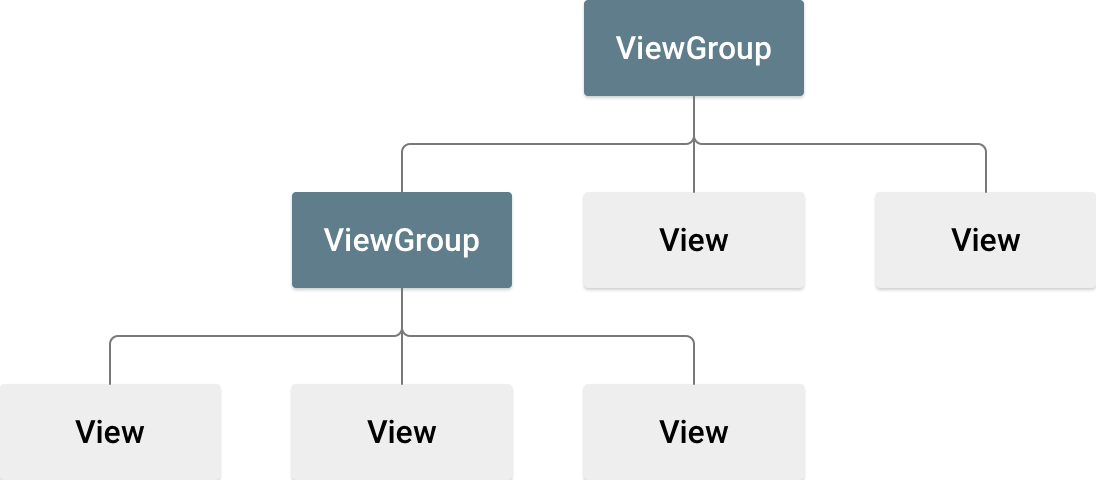
\includegraphics[width=12cm]{ViewGroup.png}
						\centering
						\caption{Illustration of a view hierarchy, which defines a UI layout}
						\label{fig:View}
					\end{figure}
					A layout defines the structure for a user interface in your app, such as in an activity. All elements in the layout are built using a hierarchy of View and ViewGroup objects. A View usually draws something the user can see and interact with. Whereas a ViewGroup is an invisible container that defines the layout structure for View and other ViewGroup objects, as shown in Figure~\ref{fig:View}.\\

					The View objects are usually called "widgets" and can be one of many subclasses, such as Button or TextView. The ViewGroup objects are usually called "layouts" can be one of many types that provide a different layout structure, such as LinearLayout or ConstraintLayout.\\

					You can declare a layout in two ways:
					\begin{itemize}
						\item \textbf{Declare UI elements in XML.} Android provides a straightforward XML vocabulary that corresponds to the View classes and subclasses, such as those for widgets and layouts. You can also use Android Studio's Layout Editor to build your XML layout using a drag-and-drop interface.
						\item \textbf{Instantiate layout elements at runtime.} Your app can create View and ViewGroup objects (and manipulate their properties) programmatically.
					\end{itemize}

					Declaring your UI in XML allows you to separate the presentation of your app from the code that controls its behavior. Using XML files also makes it easy to provide different layouts for different screen sizes and orientations.\\

					The Android framework gives you the flexibility to use either or both of these methods to build your app's UI. For example, you can declare your app's default layouts in XML, and then modify the layout at runtime.

				\subsubsection{Notification Overviews}
					A notification is a message that Android displays outside your app's UI to provide the user with reminders, communication from other people, or other timely information from your app. Users can tap the notification to open your app or take an action directly from the notification.\\

					Notifications appear to users in different locations and formats, such as an icon in the status bar, a more detailed entry in the notification drawer, as a badge on the app's icon, and on paired wearables automatically. When you issue a notification, it first appears as an icon in the status bar. Users can swipe down on the status bar to open the notification drawer, where they can view more details and take actions with the notification. Users can drag down on a notification in the drawer to reveal the expanded view, which shows additional content and action buttons, if provided. A notification remains visible in the notification drawer until dismissed by the app or the user.
			
				\subsubsection{Dialogs}
					A dialog is a small window that prompts the user to make a decision or enter additional information. A dialog does not fill the screen and is normally used for modal events that require users to take an action before they can proceed. The Dialog class is the base class for dialogs, but you should avoid instantiating Dialog directly. Instead, use one of the following subclasses:
					\begin{itemize}
						\item \textbf{AlertDialog:} A dialog that can show a title, up to three buttons, a list of selectable items, or a custom layout.
						\item \textbf{DatePickerDialog} or \textbf{TimePickerDialog:} A dialog with a pre-defined UI that allows the user to select a date or time.
					\end{itemize}
					
					These classes define the style and structure for your dialog, but you should use a DialogFragment as a container for your dialog. The DialogFragment class provides all the controls you need to create your dialog and manage its appearance, instead of calling methods on the Dialog object.\\

					Using DialogFragment to manage the dialog ensures that it correctly handles lifecycle events such as when the user presses the Back button or rotates the screen. The DialogFragment class also allows you to reuse the dialog's UI as an embeddable component in a larger UI, just like a traditional Fragment (such as when you want the dialog UI to appear differently on large and small screens).
			
				\subsubsection{Menus}
					Menus are a common user interface component in many types of applications. To provide a familiar and consistent user experience, you should use the Menu APIs to present user actions and other options in your activities.

				\subsubsection{Toasts}
					A toast provides simple feedback about an operation in a small popup. It only fills the amount of space required for the message and the current activity remains visible and interactive. Toasts automatically disappear after a timeout.
			\subsection{Back-end Features}
					The back-end for an Android application comprises mainly of the the programming languages along with the various APIs (Application Programming Interfaces) provided along with the many Android Studio libraries. Few of the APIs that are used in this project are the TensorFlow Lite APIs, Firebase APIs, Google Text-to-Speech APIs and the Google Speech-to-Text APIs. Each of these APIs are discussed in further detail in the subsequent sections.\\

					Few of the key Backend Features required by the Android Application are listed below:
					\begin{itemize}
						\item Intents and Intent Filters
						\item Data and File Storage
						\item App Resources
						\item Permissions
					\end{itemize}
					\subsubsection{Intents and Intent Filters}
						\begin{figure}[b]
							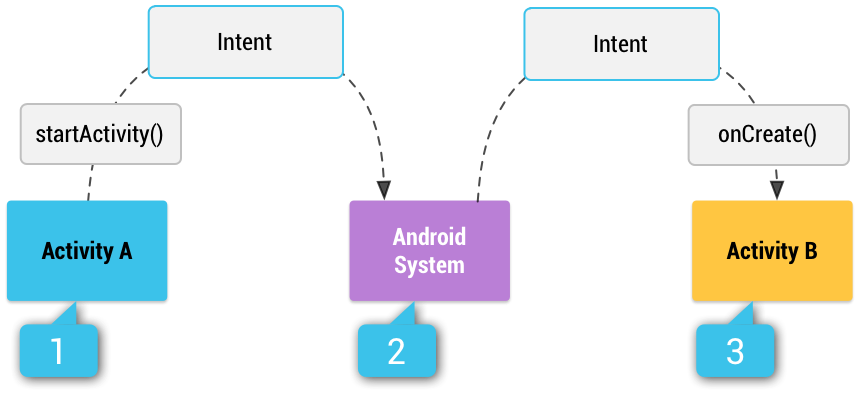
\includegraphics[width=12cm]{IntentFilters.png}
							\centering
							\caption{Illustration of how an implicit intent is delivered through the system to start another activity}
							\label{fig:IntentFilters}
						\end{figure}
						An Intent is a messaging object you can use to request an action from another app component. Although intents facilitate communication between components in several ways, there are three fundamental use cases:
						\begin{itemize}
							\item \textbf{Starting an activity:} An Activity represents a single screen in an app. You can start a new instance of an Activity by passing an Intent to startActivity(). The Intent describes the activity to start and carries any necessary data. If you want to receive a result from the activity when it finishes, call startActivityForResult(). Your activity receives the result as a separate Intent object in your activity's onActivityResult() callback.
							\item \textbf{Starting a service:} A Service is a component that performs operations in the background without a user interface. With Android 5.0 (API level 21) and later, you can start a service with JobScheduler. For versions earlier than Android 5.0 (API level 21), you can start a service by using methods of the Service class. You can start a service to perform a one-time operation (such as downloading a file) by passing an Intent to startService(). The Intent describes the service to start and carries any necessary data. If the service is designed with a client-server interface, you can bind to the service from another component by passing an Intent to bindService().
							\item \textbf{Delivering a broadcast: } A broadcast is a message that any app can receive. The system delivers various broadcasts for system events, such as when the system boots up or the device starts charging. You can deliver a broadcast to other apps by passing an Intent to sendBroadcast() or sendOrderedBroadcast().
						\end{itemize}

						There are two types of Intents - Implicit and Explicit Intents.
						\begin{itemize}
							\item \textbf{Explicit intents} specify which application will satisfy the intent, by supplying either the target app's package name or a fully-qualified component class name. You'll typically use an explicit intent to start a component in your own app, because you know the class name of the activity or service you want to start. For example, you might start a new activity within your app in response to a user action, or start a service to download a file in the background.
							\item \textbf{Implicit intents} do not name a specific component, but instead declare a general action to perform, which allows a component from another app to handle it. For example, if you want to show the user a location on a map, you can use an implicit intent to request that another capable app show a specified location on a map.
						\end{itemize}

						Figure~\ref{fig:IntentFilters}  shows how an intent is used when starting an activity. When the Intent object names a specific activity component explicitly, the system immediately starts that component.\\

						When you use an implicit intent, the Android system finds the appropriate component to start by comparing the contents of the intent to the intent filters declared in the manifest file of other apps on the device. If the intent matches an intent filter, the system starts that component and delivers it the Intent object. If multiple intent filters are compatible, the system displays a dialog so the user can pick which app to use.\\

						An intent filter is an expression in an app's manifest file that specifies the type of intents that the component would like to receive. For instance, by declaring an intent filter for an activity, you make it possible for other apps to directly start your activity with a certain kind of intent. Likewise, if you do not declare any intent filters for an activity, then it can be started only with an explicit intent.

					\subsubsection{Data and File Storage}
					Android uses a file system that's similar to disk-based file systems on other platforms. The system provides several options for you to save your app data:
					\begin{itemize}
						\item \textbf{App-specific storage:} Store files that are meant for your app's use only, either in dedicated directories within an internal storage volume or different dedicated directories within external storage. Use the directories within internal storage to save sensitive information that other apps shouldn't access.
						\item \textbf{Shared storage:} Store files that your app intends to share with other apps, including media, documents, and other files.
						\item \textbf{Preferences:} Store private, primitive data in key-value pairs.
						\item \textbf{Databases:} Store structured data in a private database using the Room persistence library.
					\end{itemize}

					The solution you choose depends on your specific needs:\\

					\textbf{How much space does your data require?} Internal storage has limited space for app-specific data. Use other types of storage if you need to save a substantial amount of data.\\

					\textbf{How reliable does data access need to be?} If your app's basic functionality requires certain data, such as when your app is starting up, place the data within internal storage directory or a database. App-specific files that are stored in external storage aren't always accessible because some devices allow users to remove a physical device that corresponds to external storage.\\

					\textbf{What kind of data do you need to store?} If you have data that's only meaningful for your app, use app-specific storage. For shareable media content, use shared storage so that other apps can access the content. For structured data, use either preferences (for key-value data) or a database (for data that contains more than 2 columns).\\
					
					\textbf{Should the data be private to your app?} When storing sensitive data—data that shouldn't be accessible from any other app—use internal storage, preferences, or a database. Internal storage has the added benefit of the data being hidden from users.\newline \newline

					Android provides two types of physical storage locations: internal storage and external storage. On most devices, internal storage is smaller than external storage. However, internal storage is always available on all devices, making it a more reliable place to put data on which your app depends.\\
					
					Removable volumes, such as an SD card, appear in the file system as part of external storage. Android represents these devices using a path, such as /sdcard. Apps themselves are stored within internal storage by default.			
				
				\subsubsection{App Resources}
					Resources are the additional files and static content that your code uses, such as bitmaps, layout definitions, user interface strings, animation instructions, and more.\\

					You should always externalize app resources such as images and strings from your code, so that you can maintain them independently. You should also provide alternative resources for specific device configurations, by grouping them in specially-named resource directories. At runtime, Android uses the appropriate resource based on the current configuration. For example, you might want to provide a different UI layout depending on the screen size or different strings depending on the language setting.\\
					
					Once you externalize your app resources, you can access them using resource IDs that are generated in your project's R class.

				\subsubsection{Premissions}
					The purpose of a permission is to protect the privacy of an Android user. Android apps must request permission to access sensitive user data (such as contacts and SMS), as well as certain system features (such as camera and internet). Depending on the feature, the system might grant the permission automatically or might prompt the user to approve the request.\\

					A central design point of the Android security architecture is that no app, by default, has permission to perform any operations that would adversely impact other apps, the operating system, or the user. This includes reading or writing the user's private data (such as contacts or emails), reading or writing another app's files, performing network access, keeping the device awake, and so on.\\

					An app must publicize the permissions it requires by including <uses-permission> tags in the app manifest. If your app lists normal permissions in its manifest (that is, permissions that don't pose much risk to the user's privacy or the device's operation), the system automatically grants those permissions to your app.\\

					If your app lists dangerous permissions in its manifest (that is, permissions that could potentially affect the user's privacy or the device's normal operation), the user must explicitly agree to grant those permissions.
		\section{Inception v3 Neural Network}
			Inception v3 is a widely-used image recognition model that has been shown to attain greater than 78.1\% accuracy on the ImageNet dataset. The model is the culmination of many ideas developed by multiple researchers over the years. It is based on the original paper: "Rethinking the Inception Architecture for Computer Vision" by Szegedy, et. al.\\

			The model itself is made up of symmetric and asymmetric building blocks, including convolutions, average pooling, max pooling, concats, dropouts, and fully connected layers. Batchnorm is used extensively throughout the model and applied to activation inputs. Loss is computed via Softmax.\\
			\begin{figure}[h]
				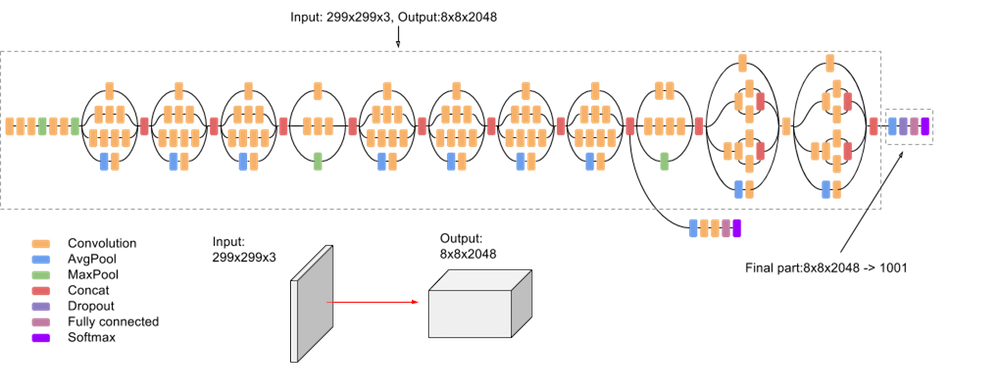
\includegraphics[width=\textwidth]{inceptionover.png}
				\centering
				\caption{Inception v3 Model Overview}
				\label{fig:IncOver}
			\end{figure}

			A high-level diagram of the model is shown in Figure~\ref{fig:IncOver}.

			\subsubsection{Estimator API}
			The TPU version of Inception v3 is written using TPUEstimator, an API designed to facilitate development, so that you can focus on the models themselves rather than on the details of the underlying hardware. The API does most of the low-level grunge work necessary for running models on TPUs behind the scenes, while automating common functions, such as saving and restoring checkpoints.\\

			The Estimator API enforces separation of model and input portions of the code. You have to define model\_fn and input\_fn functions, corresponding to model definition and input pipeline / preprocessing stages of the TensorFlow graph, respectively. Below is a sample skeleton of these functions:\\
			\begin{lstlisting}[language=Python]
def model_fn(features, labels, mode, params):
	...
return tpu_estimator.TPUEstimatorSpec(mode=mode, loss=loss, train_op=train_op)

def input_fn(params):
	def parser(serialized_example):
		...
		return image, label

	...
images, labels = dataset.make_one_shot_iterator().get_next()
return images, labels
			\end{lstlisting}
			Two key functions provided by the API are train() and evaluate() used to train and evaluate, respectively. These are usually called somewhere in the main function. An example of this is shown below:\\
			\begin{lstlisting}[language=Python]
def main(unused_argv):
...
run_config = tpu_config.RunConfig(
	master=FLAGS.master,
	model_dir=FLAGS.model_dir,
	session_config=tf.ConfigProto(
		allow_soft_placement=True, log_device_placement=True),
	tpu_config=tpu_config.TPUConfig(FLAGS.iterations, FLAGS.num_shards),)
 
estimator = tpu_estimator.TPUEstimator(
	model_fn=model_fn,
	use_tpu=FLAGS.use_tpu,
	train_batch_size=FLAGS.batch_size,
	eval_batch_size=FLAGS.batch_size,
	config=run_config)
			  
estimator.train(input_fn=input_fn, max_steps=FLAGS.train_steps)
			  
eval_results = inception_classifier.evaluate(
	input_fn=imagenet_eval.input_fn, steps=eval_steps)
			\end{lstlisting}
			\subsubsection{ImageNet Dataset}
			Before the model can be used to recognize images, it must be trained. This is usually done via supervised learning using a large set of labeled images. Although Inception v3 can be trained from many different labeled image sets, ImageNet is a common dataset of choice.\\

			ImageNet has over ten million URLs of labeled images. About a million of the images also have bounding boxes specifying a more precise location for the labeled objects.\\
			
			For this model, the ImageNet dataset is composed of 1,331,167 images which are split into training and evaluation datasets containing 1,281,167 and 50,000 images, respectively.\\
			
			The training and evaluation datasets are kept separate intentionally. Only images from the training dataset are used to train the model and only images from the evaluation dataset are used to evaluate model accuracy.\\
			
			The model expects images to be stored as TFRecords. To convert images from raw JPEG files into TFRecords, use the open source batch script: download\_and\_preprocess\_imagenet.sh. The script should produce a series of files (for both training and validation) of the form:\\
			\begin{lstlisting}[language=Python]
${DATA_DIR}/train-00000-of-01024
${DATA_DIR}/train-00001-of-01024
 ...
${DATA_DIR}/train-01023-of-01024
and
${DATA_DIR}/validation-00000-of-00128
${DATA_DIR}/validation-00001-of-00128
 ...
${DATA_DIR}/validation-00127-of-00128
			\end{lstlisting}
			where DATA\_DIR is the location where the set resides, for example: \\ DATA\_DIR=\$HOME/imagenet-data.
		
			\subsubsection{Input Pipeline}
				Each Cloud TPU device has 8 cores and is connected to a host (CPU). Larger slices have multiple hosts. Other larger configurations interact with multiple hosts. For instance, v2-256 communicates with 16 hosts.\\
				\begin{figure}[h]
					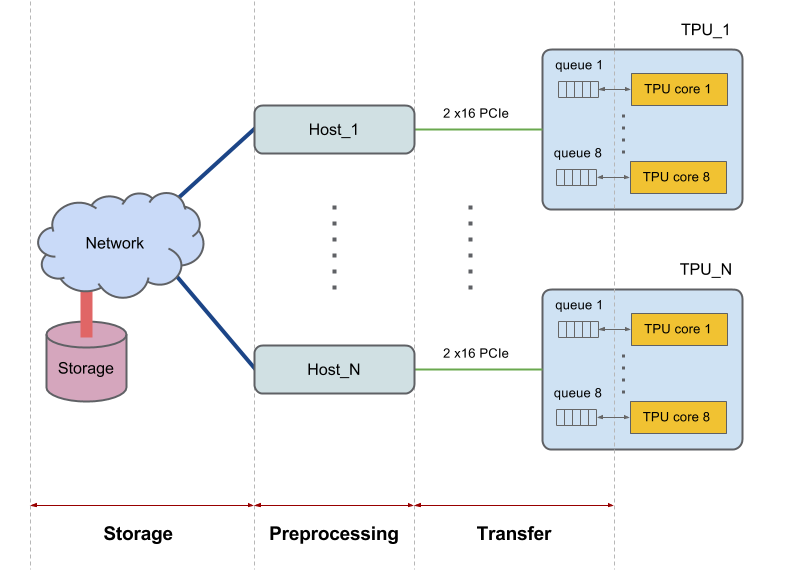
\includegraphics[width=\textwidth]{InputPipe.png}
					\centering
					\caption{Inception v3 Input Pipeline}
					\label{fig:InputPipe}
				\end{figure}

				Hosts retrieve data from the file system or local memory, do whatever data preprocessing is required, and then transfer preprocessed data to the TPU cores. We consider these three phases of data handling done by the host individually and refer to the phases as: 1) Storage, 2) Preprocessing, 3) Transfer. A high level picture of the diagram is shown in Figure~\ref{fig:InputPipe}.\\
				\begin{figure}[h]
					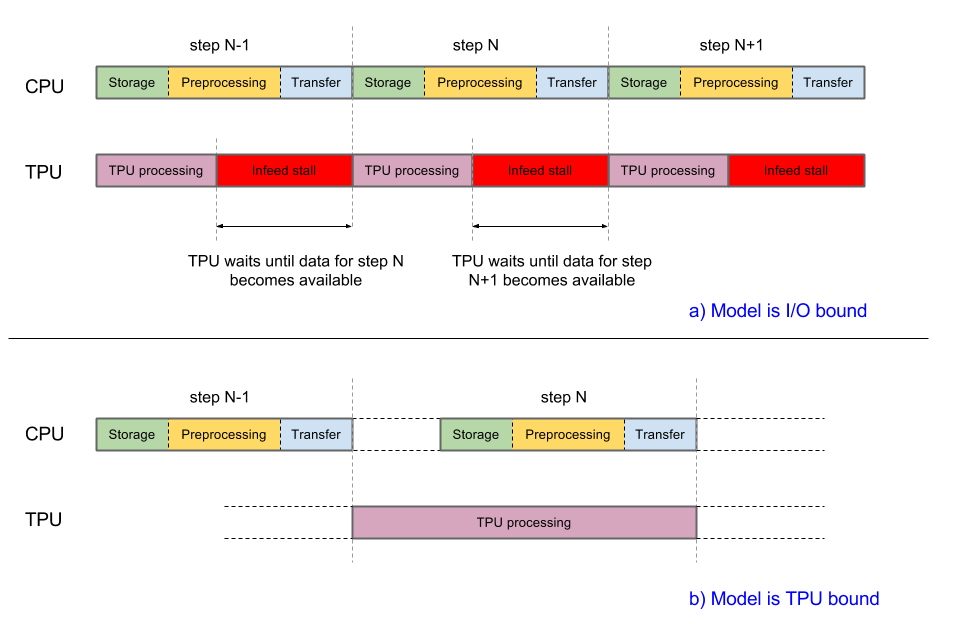
\includegraphics[width=\textwidth]{PerfModel.png}
					\centering
					\caption{Inception v3 Performance Models}
					\label{fig:PerfModel}
				\end{figure}

				To yield good performance, the system should be balanced. Whatever amount of time a host CPU spends retrieving images, decoding them, and doing relevant preprocessing, should ideally be slightly less or about the same as that spent by the TPU doing computations. If the host CPU takes longer than the TPU to complete the three data handling phases, then execution will be host bound. (Note: because TPUs are so fast, this may be unavoidable for some very simple models.) Both cases are shown in the Figure~\ref{fig:PerfModel}.\\
		
				The current implementation of Inception v3 lives right at the edge of being input-bound. Images have to be retrieved from the file system, decoded, and then preprocessed. Different types of preprocessing stages are available, ranging from moderate to complex. If we use the most complex of preprocessing stages, the large number of expensive operations executed by the preprocessing stage will push the system over the edge and the training pipeline will be preprocessing bound. However, it is not necessary to resort to that level of complexity to attain greater than 78.1\% accuracy, and we instead use a moderately complex preprocessing stage that tilts the scale in the other direction and keeps the model TPU-bound. This is discussed in more detail in the next section.\\

				The model uses tf.data.Dataset to handle all input pipeline related needs. See the datasets performance guide for more information on how to optimize input pipelines using the tf.data API.\\

				Although you can simply define a function and pass it to the Estimator API, in the case of Inception, create class InputPipeline encapsulates all required functionality and define a \_\_call\_\_ method instead.\\

				The Estimator API makes it very straightforward to use this class. One simply has to pass it to the input\_fn parameter of functions train() and evaluate(), as shown in the sample code snippet below:\\
				\begin{lstlisting}[language=Python]
def main(unused_argv):

...

  inception_classifier = tpu_estimator.TPUEstimator(
      model_fn=inception_model_fn,
      use_tpu=FLAGS.use_tpu,
      config=run_config,
      params=params,
      train_batch_size=FLAGS.train_batch_size,
      eval_batch_size=eval_batch_size,
      batch_axis=(batch_axis, 0))

          ...

  for cycle in range(FLAGS.train_steps // FLAGS.train_steps_per_eval):
    tf.logging.info('Starting training cycle %d.' % cycle)
    inception_classifier.train(
        input_fn=InputPipeline(True), steps=FLAGS.train_steps_per_eval)

    tf.logging.info('Starting evaluation cycle %d .' % cycle)
    eval_results = inception_classifier.evaluate(
        input_fn=InputPipeline(False), steps=eval_steps, hooks=eval_hooks)
    tf.logging.info('Evaluation results: %s' % eval_results)
				\end{lstlisting}

				The main elements of class InputPipeline are shown in the code snippet below, where we have highlighted the three phases with different colors. Method \_\_call\_\_ creates the dataset using tf.data.Dataset and then makes a series of API calls to utilize the built-in prefetch, interleave, and shuffling capabilities of the dataset.\\
				\begin{lstlisting}[language=Python]
class InputPipeline(object):

  def __init__(self, is_training):
    self.is_training = is_training

  def __call__(self, params):
    # Storage
    file_pattern = os.path.join(
        FLAGS.data_dir, 'train-*' if self.is_training else 'validation-*')
    dataset = tf.data.Dataset.list_files(file_pattern)
    if self.is_training and FLAGS.initial_shuffle_buffer_size > 0:
      dataset = dataset.shuffle(
          buffer_size=FLAGS.initial_shuffle_buffer_size)
    if self.is_training:
      dataset = dataset.repeat()

    def prefetch_dataset(filename):
      dataset = tf.data.TFRecordDataset(
          filename, buffer_size=FLAGS.prefetch_dataset_buffer_size)
      return dataset

    dataset = dataset.apply(
        tf.contrib.data.parallel_interleave(
            prefetch_dataset,
            cycle_length=FLAGS.num_files_infeed,
            sloppy=True))
    if FLAGS.followup_shuffle_buffer_size > 0:
      dataset = dataset.shuffle(
          buffer_size=FLAGS.followup_shuffle_buffer_size)

    # Preprocessing
    dataset = dataset.map(
        self.dataset_parser,
        num_parallel_calls=FLAGS.num_parallel_calls)

    dataset = dataset.prefetch(batch_size)
    dataset = dataset.apply(
        tf.contrib.data.batch_and_drop_remainder(batch_size))
    dataset = dataset.prefetch(2)  # Prefetch overlaps in-feed with training
    images, labels = dataset.make_one_shot_iterator().get_next()

    # Transfer
    return images, labels
				\end{lstlisting}

				The storage section begins with the creation of a dataset and includes the reading of TFRecords from storage (using tf.data.TFRecordDataset). Special purpose functions repeat() and shuffle() are used as needed. Function tf.contrib.data.parallel\_interleave() maps function prefetch\_dataset() across its input to produce nested datasets, and outputs their elements interleaved. It gets elements from cycle\_length nested datasets in parallel, which increases throughput. The sloppy argument relaxes the requirement that the outputs be produced in a deterministic order, and allows the implementation to skip over nested datasets whose elements are not readily available when requested.\\

				The preprocessing section calls dataset.map(parser) which in turn calls the parser function where images are preprocessed. The details of the preprocessing stage are discussed in the next section.\\

				The transfer section (at the end of the function) includes the line return images, labels. TPUEstimator takes the returned values and automatically transfers them to the device.\\
				\begin{figure}[h]
					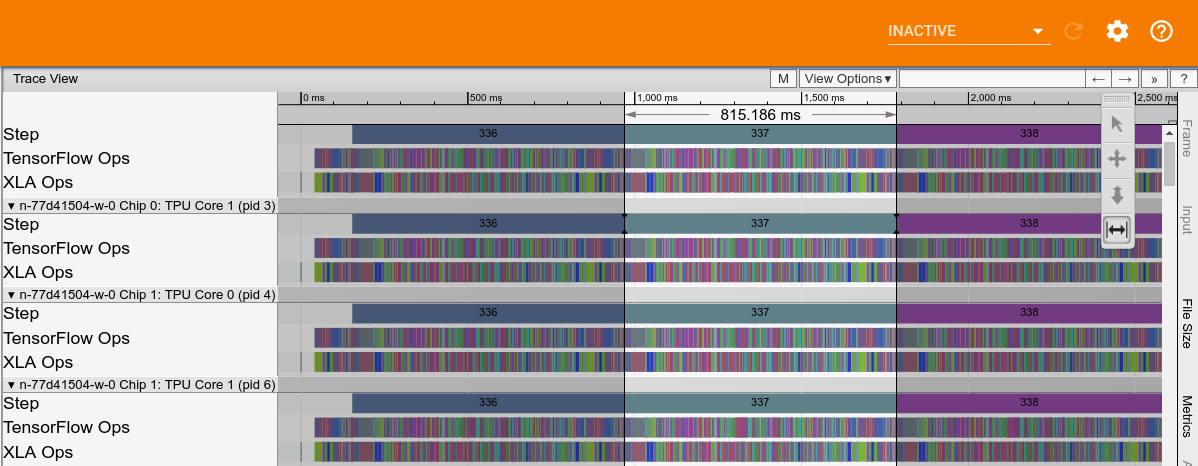
\includegraphics[width=\textwidth]{TPUInception.png}
					\centering
					\caption{Sample Cloud TPU Performance Trace of Inception v3}
					\label{fig:TPUInception}
				\end{figure}

				Figure~\ref{fig:TPUInception} shows a sample Cloud TPU performance trace of Inception v3. TPU compute time, discounting any infeeding stalls, is currently at 815 msecs or so.\\
			\subsubsection{Preprocessing Stage}
				Image preprocessing is a crucial part of the system and can heavily influence the maximum accuracy that the model attains during training. At a minimum, images need to be decoded and resized to fit the model. In the case of Inception, images need to be 299x299x3 pixels.\\

				However, simply decoding and resizing will not be enough to get good accuracy. The ImageNet training dataset contains 1,281,167 images. One pass over the set of training images is referred to as an epoch. During training, the model will require several passes through the training dataset to improve its image recognition capabilities. In the case of Inception v3, the number of epochs needed will be somewhere in the 140 to 200 range depending on the global batchsize.\\

				It is extremely beneficial to continuously alter the images before feeding them to the model and to do so in such a manner that a particular image is slightly different at every epoch. How to best do this preprocessing of images is as much art as it is science. On the one hand, a well designed preprocessing stage can significantly boost the recognition capabilities of a model. On the other, too simple a preprocessing stage may create an artificial ceiling on the maximum accuracy that the same model can attain during training.\\

				Inception v3 offers different options for the preprocessing stage, ranging from relatively simple and computationally inexpensive to fairly complex and computationally expensive. Two distinct flavors of such can be found in files vgg\_preprocessing.py and inception\_preprocessing.py.\\

				File vgg\_preprocessing.py defines a preprocessing stage that has been used successfully to train resnet to 75\% accuracy, but yields suboptimal results when applied on Inception v3.\\

				File inception\_preprocessing.py contains a multi-option preprocessing stage with different levels of complexity that has been used successfully to train Inception v3 to accuracies in the 78.1-78.5\% range when run on TPUs. This section discusses the preprocessing pipeline.\\

				Preprocessing differs depending on whether the model is undergoing training or being used for inference/evaluation.\\

				At evaluation time, preprocessing is quite straightforward: crop a central region of the image and then resize it to the default 299x299 size. The snippet code that does this is shown below:\\
				\begin{lstlisting}[language=Python]
def preprocess_for_eval(image, height, width, central_fraction=0.875):
  with tf.name_scope(scope, 'eval_image', [image, height, width]):
    if image.dtype != tf.float32:
      image = tf.image.convert_image_dtype(image, dtype=tf.float32)
    image = tf.image.central_crop(image, central_fraction=central_fraction)
    image = tf.expand_dims(image, 0)
    image = tf.image.resize_bilinear(image, [height, width], align_corners=False)
    image = tf.squeeze(image, [0])
    image = tf.subtract(image, 0.5)
    image = tf.multiply(image, 2.0)
    image.set_shape([height, width, 3])
    return image
				\end{lstlisting}				

				During training, the cropping is randomized: a bounding box is chosen randomly to select a region of the image which is then resized. The resized image is then optionally flipped and its colors are distorted. The snippet of code that does this is shown below:\\
				\begin{lstlisting}[language=Python]
def preprocess_for_train(image, height, width, bbox, fast_mode=True, scope=None):
  with tf.name_scope(scope, 'distort_image', [image, height, width, bbox]):
    if bbox is None:
      bbox = tf.constant([0.0, 0.0, 1.0, 1.0], dtype=tf.float32, shape=[1, 1, 4])
    if image.dtype != tf.float32:
      image = tf.image.convert_image_dtype(image, dtype=tf.float32)

    distorted_image, distorted_bbox = distorted_bounding_box_crop(image, bbox)
    distorted_image.set_shape([None, None, 3])

    num_resize_cases = 1 if fast_mode else 4
    distorted_image = apply_with_random_selector(
        distorted_image,
        lambda x, method: tf.image.resize_images(x, [height, width], method),
        num_cases=num_resize_cases)

    distorted_image = tf.image.random_flip_left_right(distorted_image)

    if FLAGS.use_fast_color_distort:
      distorted_image = distort_color_fast(distorted_image)
    else:
      num_distort_cases = 1 if fast_mode else 4
      distorted_image = apply_with_random_selector(
          distorted_image,
          lambda x, ordering: distort_color(x, ordering, fast_mode),
          num_cases=num_distort_cases)

    distorted_image = tf.subtract(distorted_image, 0.5)
    distorted_image = tf.multiply(distorted_image, 2.0)
    return distorted_image
				\end{lstlisting}

				Function distort\_color is in charge of color alteration. It offers a fast mode where only brightness and saturation are modified. The full mode modifies brightness, saturation, and hue, and randomly alters the order in which these get modified. A code snippet of this function is shown below:\\
				\begin{lstlisting}[language=Python]
def distort_color(image, color_ordering=0, fast_mode=True, scope=None):
  with tf.name_scope(scope, 'distort_color', [image]):
    if fast_mode:
      if color_ordering == 0:
        image = tf.image.random_brightness(image, max_delta=32. / 255.)
        image = tf.image.random_saturation(image, lower=0.5, upper=1.5)
      else:
        image = tf.image.random_saturation(image, lower=0.5, upper=1.5)
        image = tf.image.random_brightness(image, max_delta=32. / 255.)
    else:
      if color_ordering == 0:
        image = tf.image.random_brightness(image, max_delta=32. / 255.)
        image = tf.image.random_saturation(image, lower=0.5, upper=1.5)
        image = tf.image.random_hue(image, max_delta=0.2)
        image = tf.image.random_contrast(image, lower=0.5, upper=1.5)
      elif color_ordering == 1:
        image = tf.image.random_saturation(image, lower=0.5, upper=1.5)
        image = tf.image.random_brightness(image, max_delta=32. / 255.)
        image = tf.image.random_contrast(image, lower=0.5, upper=1.5)
        image = tf.image.random_hue(image, max_delta=0.2)
      elif color_ordering == 2:
        image = tf.image.random_contrast(image, lower=0.5, upper=1.5)
        image = tf.image.random_hue(image, max_delta=0.2)
        image = tf.image.random_brightness(image, max_delta=32. / 255.)
        image = tf.image.random_saturation(image, lower=0.5, upper=1.5)
      elif color_ordering == 3:
        image = tf.image.random_hue(image, max_delta=0.2)
        image = tf.image.random_saturation(image, lower=0.5, upper=1.5)
        image = tf.image.random_contrast(image, lower=0.5, upper=1.5)
        image = tf.image.random_brightness(image, max_delta=32. / 255.)

    return tf.clip_by_value(image, 0.0, 1.0)
				\end{lstlisting}

				Function distort\_color is computationally expensive, partly due to the nonlinear RGB to HSV and HSV to RGB conversions that are required in order to access hue and saturation. Both fast and full modes require these conversions and although fast mode is less computationally expensive, it still pushes the model to the CPU-compute-bound region, when enabled.\\

				As an alternative, a new function distort\_color\_fast has been added to the list of options. This function maps the image from RGB to YCrCb using the JPEG conversion scheme and randomly alters brightness and the Cr/Cb chromas before mapping back to RGB. The function is shown in the code snippet below:\\
				\begin{lstlisting}[language=Python]
def distort_color_fast(image, scope=None):
  with tf.name_scope(scope, 'distort_color', [image]):
    br_delta = random_ops.random_uniform([], -32./255., 32./255., seed=None)
    cb_factor = random_ops.random_uniform(
        [], -FLAGS.cb_distortion_range, FLAGS.cb_distortion_range, seed=None)
    cr_factor = random_ops.random_uniform(
        [], -FLAGS.cr_distortion_range, FLAGS.cr_distortion_range, seed=None)

    channels = tf.split(axis=2, num_or_size_splits=3, value=image)
    red_offset = 1.402 * cr_factor + br_delta
    green_offset = -0.344136 * cb_factor - 0.714136 * cr_factor + br_delta
    blue_offset = 1.772 * cb_factor + br_delta
    channels[0] += red_offset
    channels[1] += green_offset
    channels[2] += blue_offset
    image = tf.concat(axis=2, values=channels)
    image = tf.clip_by_value(image, 0., 1.)
    return image
				\end{lstlisting}

				\begin{figure}[h]
					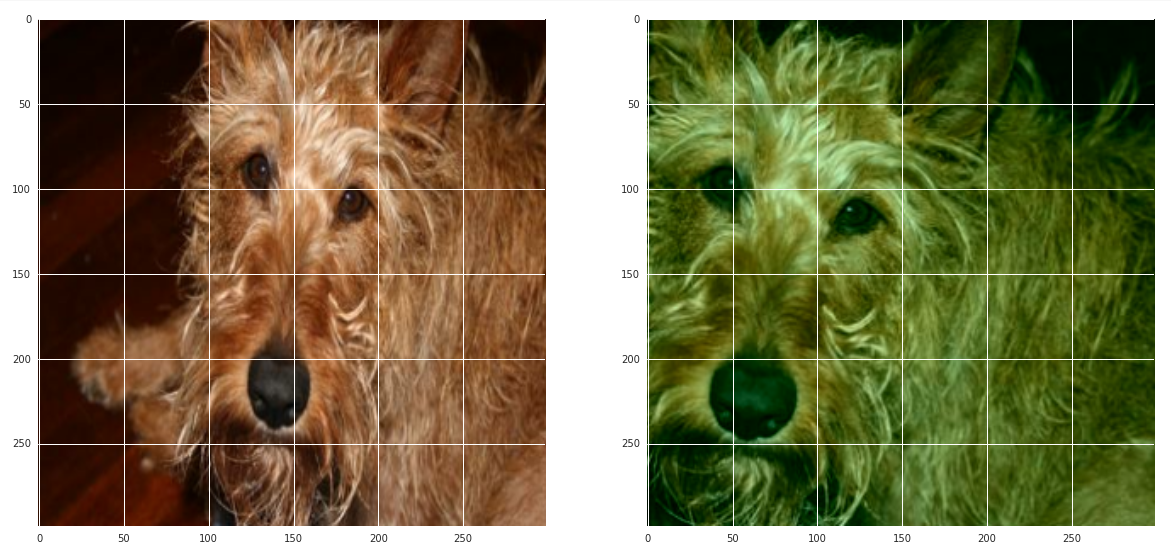
\includegraphics[width=13cm]{DistortSample.png}
					\centering
					\caption{Preprocessing Sample Image}
					\label{fig:DistortSample}
				\end{figure}

				Figure~\ref{fig:DistortSample} depicts a sample image that has undergone preprocessing. A randomly chosen region of the image has been selected and colors altered using the distort\_color\_fast function.\\

				Function distort\_color\_fast is computationally efficient and still allows training to be TPU execution time bound. In addition, it yields good results and has been used successfully to train the Inception v3 model to greater than 78.1\% accuracy using batchsizes in the 1,024 to 16,384 range. It is used as the default choice for Inception v3.\\

			\subsubsection{Learning Rate Adaptation}
				As batch sizes become larger, training becomes more difficult. Different techniques continue to be proposed to allow efficient training for large batch sizes.\\
				\begin{figure}[h]
					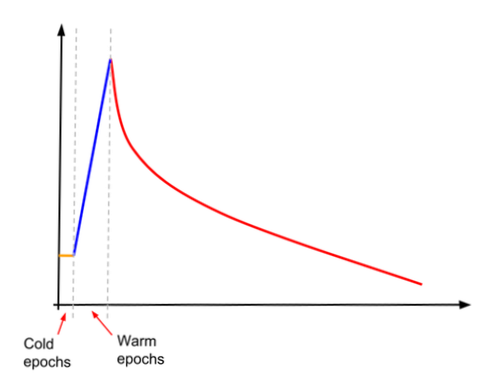
\includegraphics[width=\textwidth]{EpochIncep.png}
					\centering
					\caption{Inception v3 Learning Rate}
					\label{fig:EpochIncep}
				\end{figure}

				One of said techniques: gradual learning rate ramp-up, was used to train the model to greater than 78.1\% accuracy for batch sizes ranging from 4,096 to 16,384. For the case of inception v3, the learning rate is first set to about 10\% of what would normally be the starting learning rate. The learning rate remains constant at this low value for a specified (small) number of 'cold epochs', and then begins a linear increase for a specified number of 'warm-up epochs' at the end of which it intersects what would have been the learning rate should a normal exponential decay had been used. This is illustrated in the Figure~\ref{fig:EpochIncep}.\\

				The bit of code that does this is shown in the snippet below:\\
				\begin{lstlisting}[language=Python]
initial_learning_rate = FLAGS.learning_rate * FLAGS.train_batch_size / 256
if FLAGS.use_learning_rate_warmup:
  warmup_decay = FLAGS.learning_rate_decay**(
    (FLAGS.warmup_epochs + FLAGS.cold_epochs) /
    FLAGS.learning_rate_decay_epochs)
  adj_initial_learning_rate = initial_learning_rate * warmup_decay

final_learning_rate = 0.0001 * initial_learning_rate

train_op = None
if training_active:
  batches_per_epoch = _NUM_TRAIN_IMAGES / FLAGS.train_batch_size
  global_step = tf.train.get_or_create_global_step()
  current_epoch = tf.cast(
    (tf.cast(global_step, tf.float32) / batches_per_epoch), tf.int32)

  learning_rate = tf.train.exponential_decay(
    learning_rate=initial_learning_rate,
    global_step=global_step,
    decay_steps=int(FLAGS.learning_rate_decay_epochs * batches_per_epoch),
    decay_rate=FLAGS.learning_rate_decay,
    staircase=True)

  if FLAGS.use_learning_rate_warmup:
    wlr = 0.1 * adj_initial_learning_rate
    wlr_height = tf.cast(
      0.9 * adj_initial_learning_rate /
      (FLAGS.warmup_epochs + FLAGS.learning_rate_decay_epochs - 1),
      tf.float32)
    epoch_offset = tf.cast(FLAGS.cold_epochs - 1, tf.int32)
    exp_decay_start = (FLAGS.warmup_epochs + FLAGS.cold_epochs +
                   FLAGS.learning_rate_decay_epochs)
    lin_inc_lr = tf.add(
      wlr, tf.multiply(
        tf.cast(tf.subtract(current_epoch, epoch_offset), tf.float32),
        wlr_height))
    learning_rate = tf.where(
      tf.greater_equal(current_epoch, FLAGS.cold_epochs),
      (tf.where(tf.greater_equal(current_epoch, exp_decay_start),
              learning_rate, lin_inc_lr)),
       wlr)

  # Set a minimum boundary for the learning rate.
  learning_rate = tf.maximum(
      learning_rate, final_learning_rate, name='learning_rate')
				\end{lstlisting}
	
		\section{Application Programming Interfaces}
			An Application Programming Interfaces (API) defines functionalities that are independent of their respective implementations, which allows those implementations and definitions to vary without compromising each other. Therefore, a good API makes it easier to develop a program by providing the building blocks.\\

			When developers create code, they don’t often start from scratch. APIs enable developers can make repetitive yet complex processes highly reusable with a little bit of code. The speed that APIs enable developers to build out apps is crucial to the current pace of application development.\\

			Developers are now much more productive than they were before when they had to write a lot of code from scratch. With an API they don’t have to reinvent the wheel every time they write a new program. Instead, they can focus on the unique proposition of their applications while outsourcing all of the commodity functionality to APIs.
			\subsubsection{The principle of API abstraction enables speed and agility}
			One of the chief advantages of APIs is that they allow the abstraction of functionality between one system and another. An API endpoint decouples the consuming application from the infrastructure that provides a service. As long as the specification for what the service provider is delivering to the endpoint remains unchanged, the alterations to the infrastructure behind the endpoint should not be noticed by the applications that rely on that API.\\

			Therefore, the service provider is given a great deal of flexibility when it comes to how its services are offered. For example, if the infrastructure behind the API involves physical servers at a data center, the service provider can easily switch to virtual servers that run in the cloud.\\
			
			If the software running on those servers (such as credit card processing software) is written in, say, Java running on an Oracle-based Java application server, the service provider can migrate that to Node.js (server-side Javascript) running on Windows Azure.\\
			
			The ability of API-led connectivity to allow systems to change as easily as plugging in a plug to a socket is key to the modern vision of enterprise IT. Gone are the days of messy point-to-point integrations for connecting enterprise solutions which take time and resources to maintain.\\

			Few of the APIs used in this project are mentioned below:
			\subsection{TensorFlow Lite API}
				TensorFlow Lite is a set of tools to help developers run TensorFlow models on mobile, embedded, and IoT devices. It enables on-device machine learning inference with low latency and a small binary size.\\

				TensorFlow Lite consists of two main components:
				\begin{itemize}
					\item The TensorFlow Lite interpreter, which runs specially optimized models on many different hardware types, including mobile phones, embedded Linux devices, and microcontrollers.
					\item The TensorFlow Lite converter, which converts TensorFlow models into an efficient form for use by the interpreter, and can introduce optimizations to improve binary size and performance.
				\end{itemize}

				\subsubsection{Machine learning at the edge}
					TensorFlow Lite is designed to make it easy to perform machine learning on devices, "at the edge" of the network, instead of sending data back and forth from a server. For developers, performing machine learning on-device can help improve:
					\begin{itemize}
						\item \textbf{Latency:} There's no round-trip to a server
						\item \textbf{Privacy:} No data needs to leave the device
						\item \textbf{Connectivity:} An Internet connection isn't required
						\item \textbf{Power consumption:} Network connections are power hungry
					\end{itemize}

					TensorFlow Lite works with a huge range of devices, from tiny microcontrollers to powerful mobile phones.

				\subsubsection{Key Features}
					\begin{itemize}
						\item Interpreter tuned for on-device ML, supporting a set of core operators that are optimized for on-device applications, and with a small binary size.
						\item Diverse platform support, covering Android and iOS devices, embedded Linux, and microcontrollers, making use of platform APIs for accelerated inference.
						\item APIs for multiple languages including Java, Swift, Objective-C, C++, and Python.
						\item High performance, with hardware acceleration on supported devices, device-optimized kernels, and pre-fused activations and biases.
						\item Model optimization tools, including quantization, that can reduce size and increase performance of models without sacrificing accuracy.
						\item Efficient model format, using a FlatBuffer that is optimized for small size and portability.
						\item Pre-trained models for common machine learning tasks that can be customized to your application.
					\end{itemize}
				\subsubsection{Development Workflow}

					
					The workflow for using TensorFlow Lite involves the following steps:
					\begin{enumerate}
						\item Pick a Model
						\item Convert the Model
						\item Deploy to the Device
						\item Optimize the Model
					\end{enumerate}
					\begin{figure}[h]
						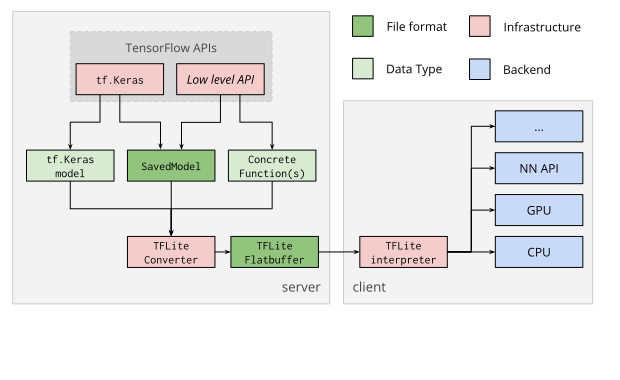
\includegraphics[width=\textwidth]{TensorWorkflow.png}
						\centering
						\caption{Workflow using TensorFlow Lite}
					\end{figure}

			\subsection{Firebase API}
				
				Firebase is a mobile and web application development platform developed by Firebase, Inc. in 2011, then acquired by Google in 2014. As of October 2018, the Firebase platform has 18 products, which are used by 1.5 million apps.\\

				The Firebase APIs provide us with a plethora of services and features that make Mobile Application Development a much simpler task. These services are discussed below.
				\begin{figure}[b]
					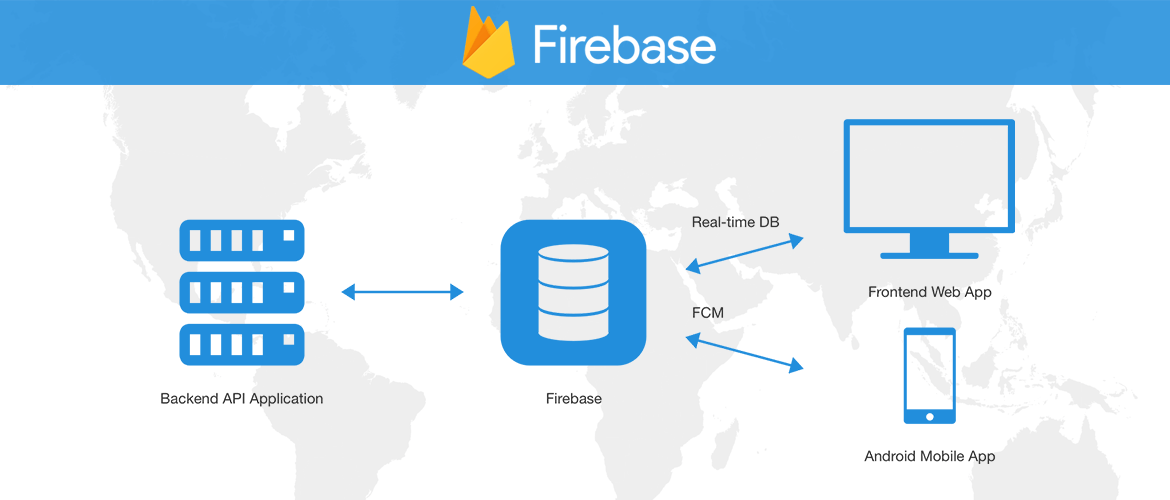
\includegraphics[width=14cm]{firebaseblog.png}
					\centering
					\caption{Firebase as a Database Server and Cloud Messaging platform}
				\end{figure}
				\subsubsection{Firebase Services}
					\begin{itemize}
						\item \textbf{Google Analytics - }Google Analytics is a cost-free app measurement solution that provides insights on app usage and user engagement.
						\item \textbf{Firebase Cloud Messaging - }Formerly known as Google Cloud Messaging (GCM), Firebase Cloud Messaging (FCM) is a cross-platform solution for messages and notifications for Android, iOS, and web applications, which as of 2016 can be used at no cost.						
						\item \textbf{Firebase Authentication - }Firebase Authentication is a service that can authenticate users using only client-side code. It supports social login providers Facebook, GitHub, Twitter and Google as well as other service providers like Google Play Games, Apple, Yahoo, and Microsoft. Additionally, it includes a user management system whereby developers can enable user authentication with email and password login stored with Firebase.
						\item \textbf{Firebase Realtime Database - }Firebase provides a real-time database and back-end as a service. The service provides application developers an API that allows application data to be synchronized across clients and stored on Firebase's cloud. The company provides client libraries that enable integration with Android, iOS, JavaScript, Java, Objective-C, Swift and Node.js applications. The database is also accessible through a REST API and bindings for several JavaScript frameworks such as AngularJS, React, Ember.js and Backbone.js. The REST API uses the Server-Sent Events protocol, which is an API for creating HTTP connections for receiving push notifications from a server. Developers using the realtime database can secure their data by using the company's server-side-enforced security rules.
						\item \textbf{Cloud Firestore - }On January 31, 2019, Cloud Firestore was officially brought out of beta, making it an official product of the Firebase lineup. It is the successor to Firebase's original databasing system, Real-time Database, and allows for nested documents and fields rather than the tree-view provided in the Real-time Database.
						\item \textbf{Firebase Storage - }Firebase Storage provides secure file uploads and downloads for Firebase apps, regardless of network quality, to be used for storing images, audio, video, or other user-generated content. It is backed by Google Cloud Storage.
						\item \textbf{Firebase Hosting - }Firebase Hosting is a static and dynamic web hosting service that launched on May 13, 2014. It supports hosting static files such as CSS, HTML, JavaScript and other files, as well as support through Cloud Functions. The service delivers files over a content delivery network (CDN) through HTTP Secure (HTTPS) and Secure Sockets Layer encryption (SSL). Firebase partners with Fastly, a CDN, to provide the CDN backing Firebase Hosting. The company states that Firebase Hosting grew out of customer requests; developers were using Firebase for its real-time database but needed a place to host their content.
						\begin{figure}[h]
							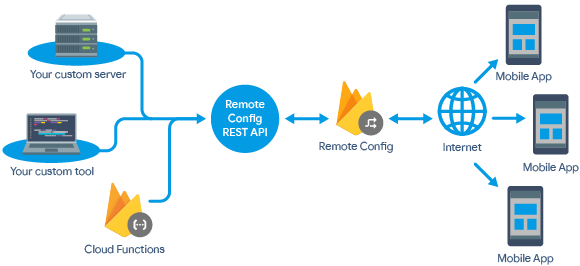
\includegraphics[width=14cm]{firebaserest.png}
							\centering
							\caption{Firebase Cloud Functions}
						\end{figure}
						\item \textbf{ML Kit - }ML Kit is a mobile machine learning system for developers launched on May 8, 2018, in beta during the Google I/O 2018. ML Kit APIs feature a variety of features including optical character recognition, detecting faces, scanning barcodes, labelling images and recognising landmarks. It is currently available for iOS or Android developers. You may also import your own TensorFlow Lite models, if the given APIs are not enough. The APIs can be used on-device or on-cloud.
						\item \textbf{Crashlytics - }Crash Reporting creates detailed reports of the errors in the app. Errors are grouped into clusters of similar stack traces and triaged by the severity of impact on app users. In addition to automatic reports, the developer can log custom events to help capture the steps leading up to a crash. Before acquiring Crashlytics, Firebase was using its own Firebase Crash Reporting.
						\item \textbf{Performance - }Firebase Performance provides insights into an app's performance and the latencies the app's users experience.
						\item \textbf{Firebase Test Lab - }Firebase Test Lab provides cloud-based infrastructure for testing Android and iOS apps in one operation. Developers can test their apps across a wide variety of devices and device configurations. Test results—including logs, videos, and screenshots—are made available in the Firebase console. Even if a developer hasn't written any test code for their app, Test Lab can exercise the app automatically, looking for crashes. Test Lab for iOS is currently in beta.
						\item \textbf{Admob - }Admob is a Google product that integrates with Firebase audience.
						\item \textbf{Firebase Dynamic Links - }Dynamic Firebase links are smart URLs that dynamically change their behavior to provide "the best available experience" across multiple platforms, including desktop web browsers, iOS, and Android, and in-depth links to mobile apps. Dynamic Links work in all app installs: if the user opens Dynamic Link on iOS or Android and the application is not installed, the user will be prompted to install the app first. Once installed, the application will start running and can access the link.
					\end{itemize}
			\subsection{Google Text-to-Speech API}
				Google Text-to-Speech is a screen reader application developed by Google for its Android operating system. It powers applications to read aloud (speak) the text on the screen with support for many languages. Text-to-Speech may be used by apps such as Google Play Books for reading books aloud, by Google Translate for reading aloud translations providing useful insight to the pronunciation of words, by Google Talkback and other spoken feedback accessibility-based applications, as well as by third-party apps. Users must install voice data for each language.
					\subsubsection{Evolution}
						\begin{figure}[b]
							\includegraphics[width=14cm]{cloudtts.png}
							\centering
							\caption{Google Text-to-Speech API}
						\end{figure}
						Some app developers have started adapting and tweaking their Android Auto apps to include Text-to-Speech, such as Hyundai in 2015. Apps such as textPlus and WhatsApp use Text-to-Speech to read notifications aloud and provide voice-reply functionality.\\
						
						Cloud Text-to-Speech is powered by WaveNet, software created by Google's UK-based AI subsidiary DeepMind. Since Google bought DeepMind in 2014, it's been exploring ways to turn the company's AI talent into tangible products. Integrating WaveNet into its cloud service is significant as Google tries to win the cloud business away from Amazon and Microsoft, presenting its AI skills as its differentiating factor.\\
						
						DeepMind's AI voice synthesis tech is notably advanced and realistic. Most voice synthesizers (including Apple's Siri) use concatenative synthesis, in which a program stores individual syllables — sounds such as “ba,” “sht,” and “oo” — and pieces them together to form words and sentences. WaveNet instead uses machine learning to generate speech. It then waveforms from a database of human speech and re-creates them at a rate of 24,000 samples per second. The end result includes voices with subtleties like lip smacks and accents. When Google first unveiled WaveNet in 2016, it was too computationally intensive to work outside of research environments, but it's since been slimmed down significantly, showing a clear pipeline from research to product. Google Cloud Text-to-Speech converts text into human-like speech in more than 180 voices across 30+ languages and variants. It applies groundbreaking research in speech synthesis (WaveNet) and Google's powerful neural networks to deliver high-fidelity audio. Includes exclusive access to WaveNet technology DeepMind has done groundbreaking research in machine learning models to generate speech that mimics human voices and sounds more natural, reducing the gap with human performance by 70\%. Cloud Text-to-Speech offers exclusive access to 90+ WaveNet voices and will continue to add more over time.
			\subsection{Google Speech-to-Text API}
				Speech recognition is an interdisciplinary subfield of computational linguistics that develops methodologies and technologies that enables the recognition and translation of spoken language into text by computers. It is also known as automatic speech recognition (ASR), computer speech recognition or speech to text (STT). It incorporates knowledge and research in the linguistics, computer science, and electrical engineering fields.\\

				Some speech recognition systems require "training" (also called "enrollment") where an individual speaker reads text or isolated vocabulary into the system. The system analyzes the person's specific voice and uses it to fine-tune the recognition of that person's speech, resulting in increased accuracy. Systems that do not use training are called "speaker independent" systems. Systems that use training are called "speaker dependent".\\
				\begin{figure}[h]
					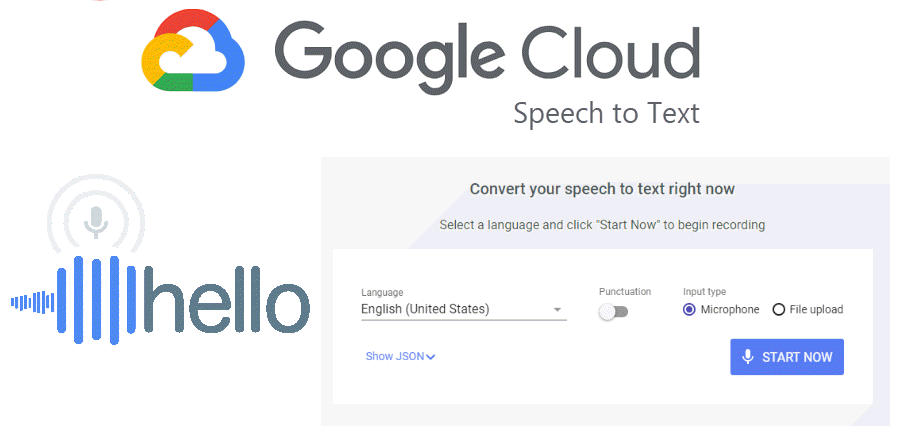
\includegraphics[width=14cm]{googlestt.png}
					\centering
					\caption{Google Speech-to-Text API}
				\end{figure}

				Speech recognition applications include voice user interfaces such as voice dialing (e.g. "call home"), call routing (e.g. "I would like to make a collect call"), domotic appliance control, search key words (e.g. find a podcast where particular words were spoken), simple data entry (e.g., entering a credit card number), preparation of structured documents (e.g. a radiology report), determining speaker characteristics, speech-to-text processing (e.g., word processors or emails), and aircraft (usually termed direct voice input).\\

				The term voice recognition or speaker identification refers to identifying the speaker, rather than what they are saying. Recognizing the speaker can simplify the task of translating speech in systems that have been trained on a specific person's voice or it can be used to authenticate or verify the identity of a speaker as part of a security process.\\
				
				From the technology perspective, speech recognition has a long history with several waves of major innovations. Most recently, the field has benefited from advances in deep learning and big data. The advances are evidenced not only by the surge of academic papers published in the field, but more importantly by the worldwide industry adoption of a variety of deep learning methods in designing and deploying speech recognition systems.\\

				For the purposes of this project, the Google Text-to-Speech API has been employed to perform the Speech Recognition operations.
	\newpage

	%Project Implementation

	\chapter{Project Implementation}\label{chapter4}
		
	\lhead{\titleref{chapter4}}
	

		\section{Project Implementation Flow}
		
				The Project Implementation Flow depicts the various stages and phases involved in the implementation of the project - starting from the input phase to the output phase. Figure~\ref{fig:ProjectFlow} depicts the various phases involved in the project implementation.\\

				As shown in the figure, the project is divided into 3 phases - The Input Phase, The Conversion and Transmission Phase and The Output Phase.
			\subsubsection{Phase I - The Input Phase}
				This phase deals with the collection of input data such as gestures (sign language), taps (for morse code) or direct speech (voice) from any client device that has the Android application installed on it.
			\subsubsection{Phase II - The Conversion and Transmission Phase}
				This phase deals with the conversion of the input data into a fundamental form (such as Morse/Digital), transmission and processing of the gathered data.
			\subsubsection{Phase III - The Output Phase}
				This phase deals with obtaining the output data from the preceding phase and represent them either visually, via vibrations or via speech, as follows:
				\begin{enumerate}
					\item Voice/Morse for the Blind
					\begin{figure}[H]
						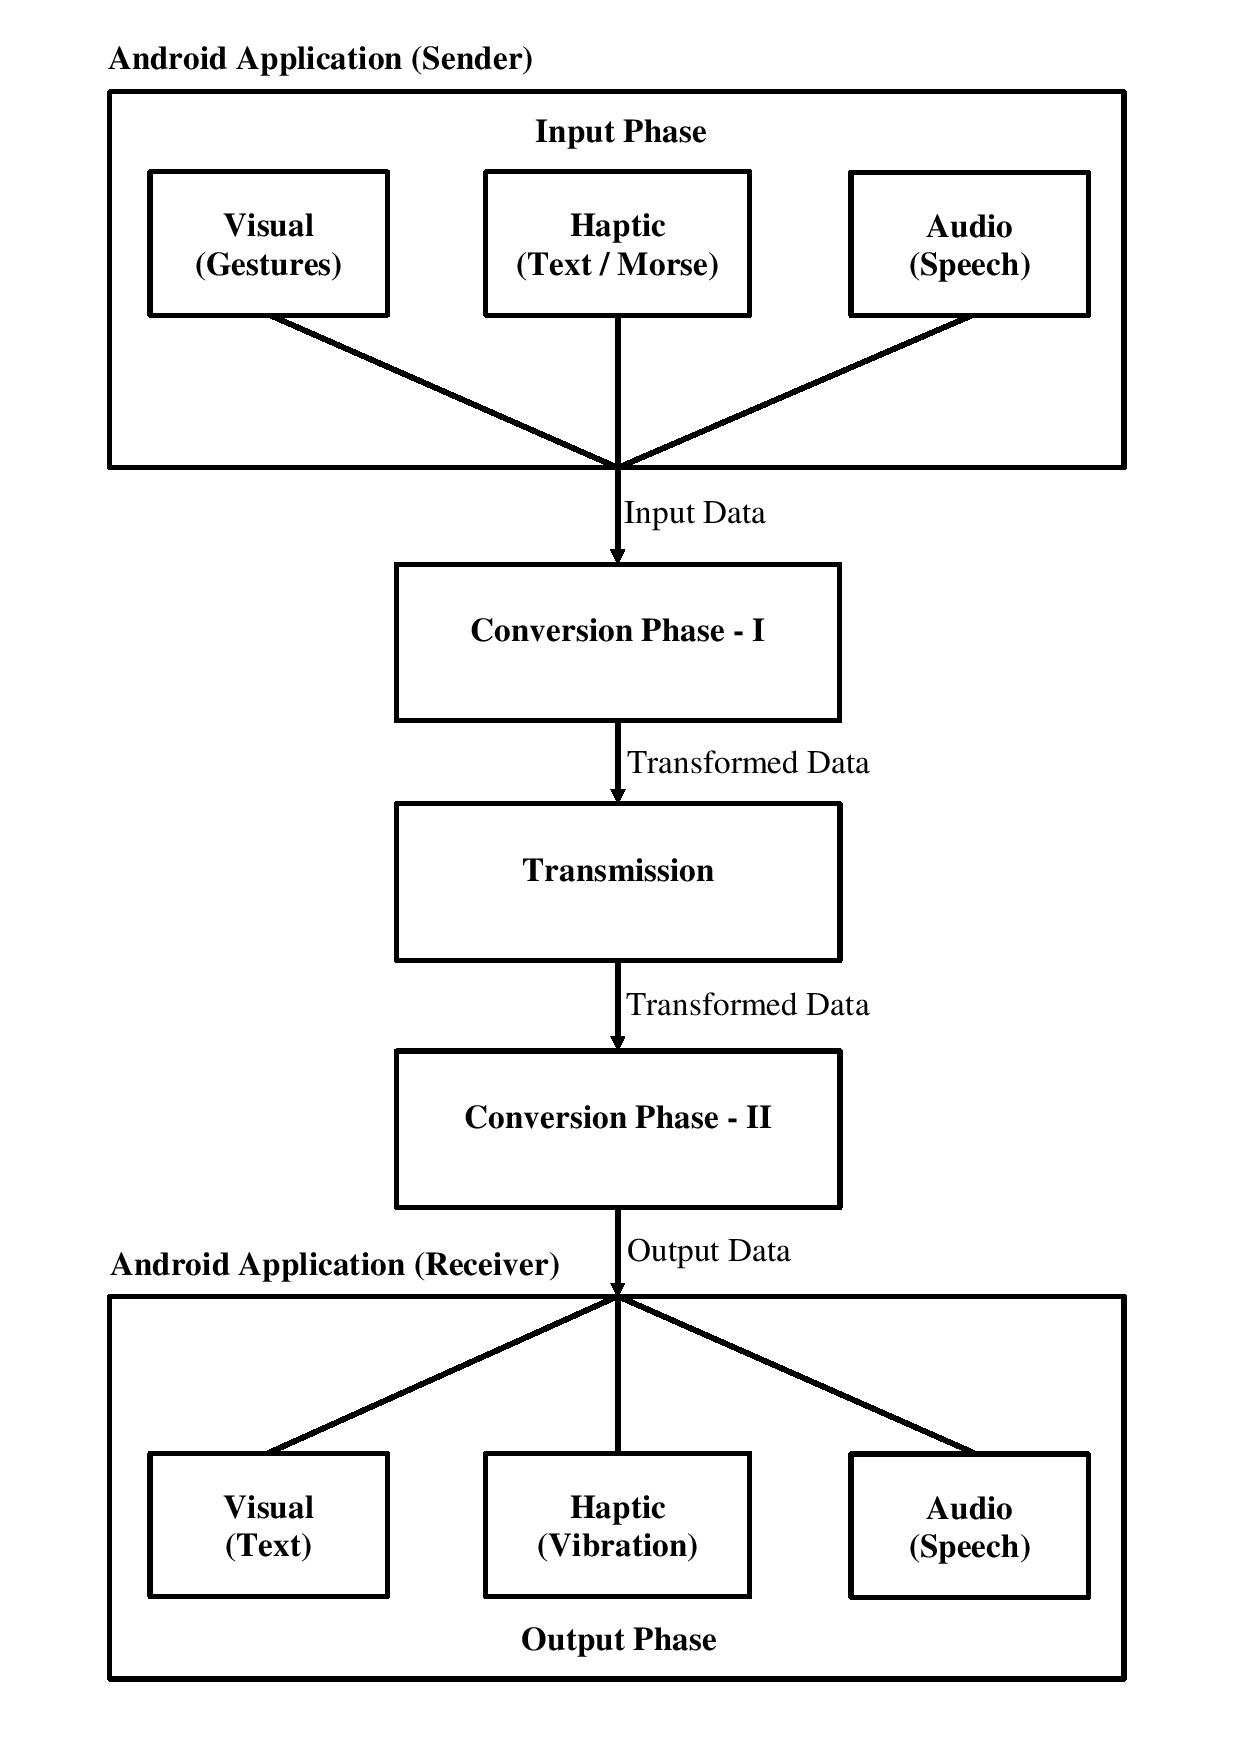
\includegraphics[width=\textwidth]{ProjectFlow.jpg}
						\centering
						\caption{Project Implementation Flowchart}
						\label{fig:ProjectFlow}
					\end{figure}
					\item Sign-language/Text for the Deaf
					\item Sign-language/Voice for the Dumb
					\item Morse codes wherever these are not possible
				\end{enumerate}
			
		\section{Android Application Implementation}
			This project uses an Android application as the front-end application to receive the user input and to generate the user output. Since the application is designed for use by the physically impaired, the various features of the application needs to be fine-tuned to cater to the target audience. The approaches used to achieve this are discussed in the subsections below.
			\subsection{Design Ideologies}
				The User Interface (UI) or User Experience (UX) of an applicaton (or any frontend software) can prove to either be very detrimental or a tremendous boost to the app usage. Since the application is designed for use by the physically-impaired, the design idealogies used play a very crucial role. Keeping this in mind, we had designed the entire applicaton focusing on easability of use and minimalism. The various design ideologies used in this project are discussed below.
				\subsubsection{Colour and Font Selection}
				\begin{figure}[h]
					\centering
					\subfloat[New Received Message]{{
\includegraphics[width=6cm]{ColourSelect.jpeg} }}%
					\qquad
					\subfloat[Previously Received Message]{{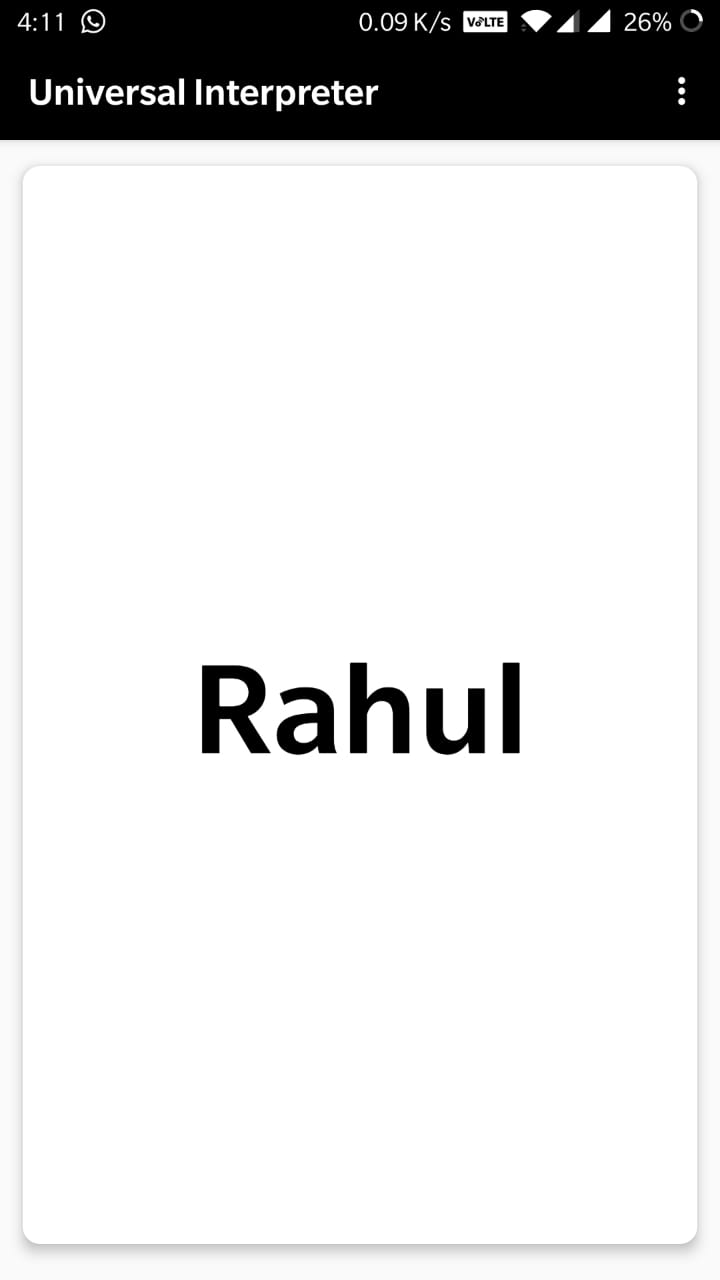
\includegraphics[width=6cm]{ReadMessage.jpeg} }}%
					\caption{Application Colour and Font Selection}%
					\label{fig:ColourSelect}%
				\end{figure}
					Keeping the concepts of minimalism and easability to read, we had decided to stick to the basic contrasting colours of black and white, with large fonts, for easability of viewing and reading.\\
					
					The new messages are depicted with a white font over a black background, and the read messages are depicted with a black font over a white background. Figure~\ref{fig:ColourSelect} represents a page of the application, portraying the colour and font selection of the application.
				\subsubsection{User-Application Interaction}
					Since the target audience of this application is the physically-impaired, we tried to limit the user-application interaction to a bare minimum. As a result, we have used two different interaction models in the application.\\

					For the landing page, the page that shows the user the list of received messages, we have used the "Two Screen Halves Model". This model enables the user to cycle through all the messages received by him/her in a clockwise or anti-clockwise manner (depending on the area of screen tapped). The 'Left Half' enables the user to either cycle through the received messages in an anti-clockwise fashion or to start a new conversation with a new user (on long tap). The 'Right Half' enables to user to either cycle through the received messages in a clockwise fashion or read the message received from the displayed user (on long tap). Figure~\ref{fig:2half} depicts the "Two Screen Halves Model".\\
					\begin{figure}[h]
						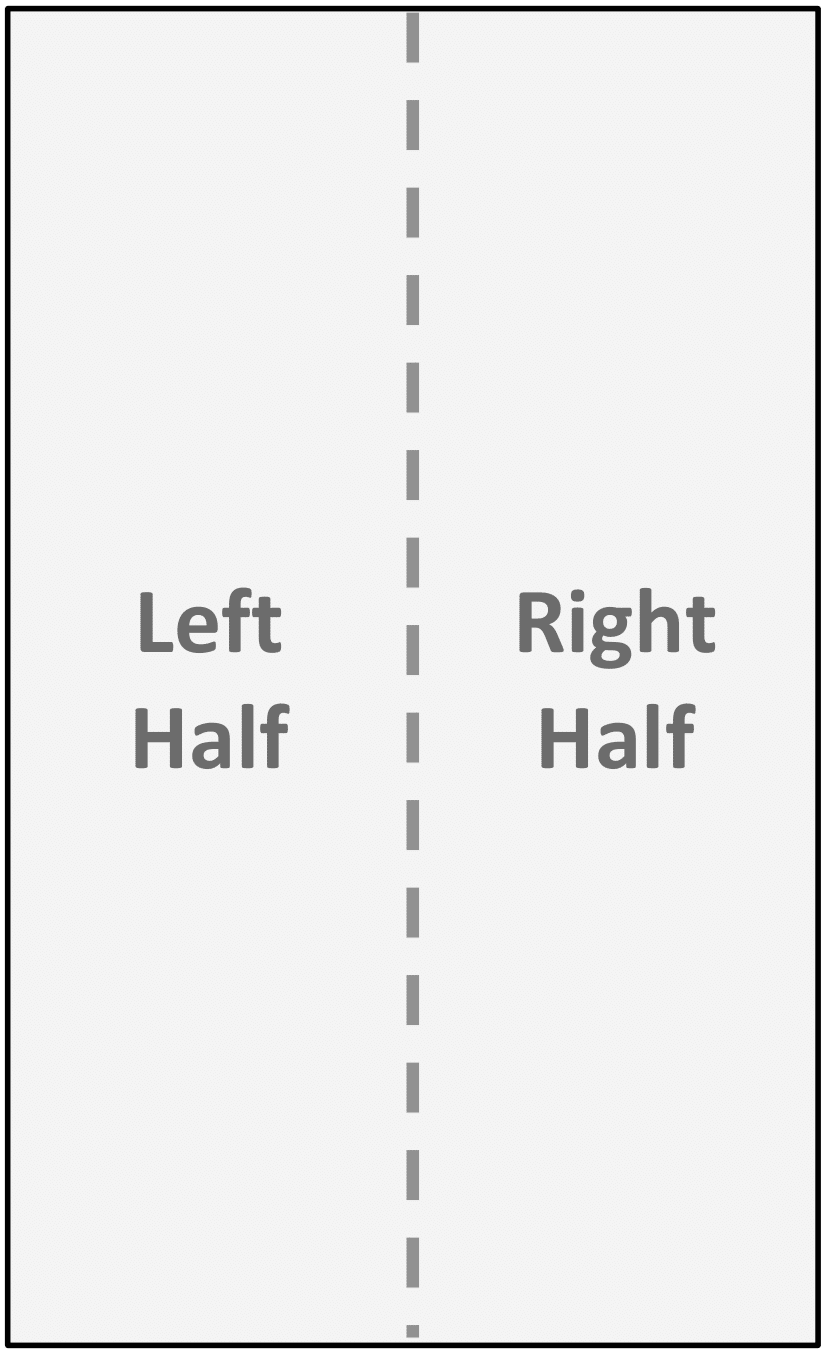
\includegraphics[width=6cm]{2half.png}
						\centering
						\caption{Two Screen Halves Model}
						\label{fig:2half}
					\end{figure} 

					Similarly, we have used the "Three Screen Halves Model" as the user-interaction model to allow the sender to input and send messages, and the receiver to read/view the input in the appropriate form. The 'Upper Left Half' is used for character deletion purposes or to use the user's camera image stream. The 'Upper Right Half' is either used to provide morse input (tap for a dot, long tap for a dash) or to use the user's camera image stream. The 'Center Area' is used either to provide a white space to the input, to use the user's camera image stream or to send the message to the desired user (on long tap). Figure~\ref{fig:3half} depicts the "Three Screen Halves Model".
					\begin{figure}[h]
						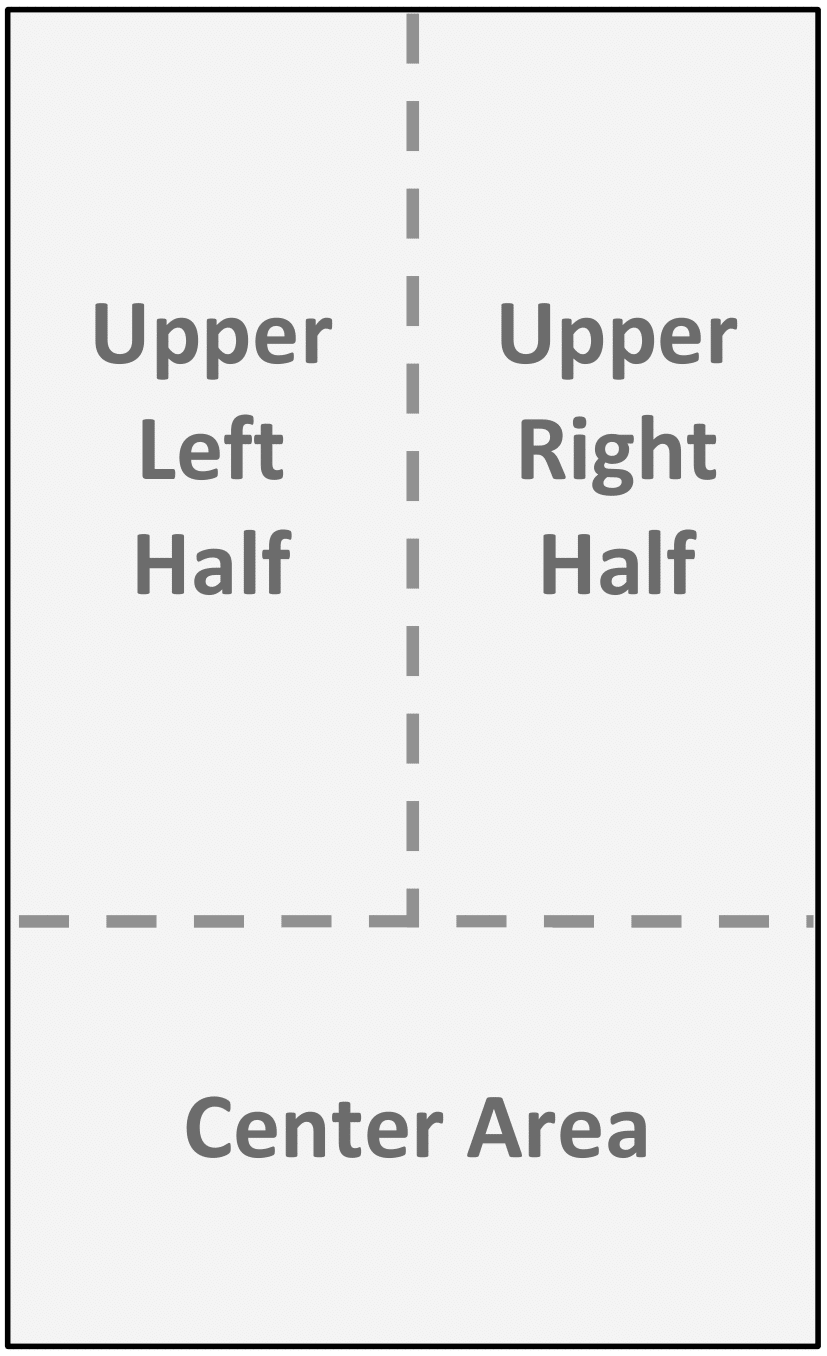
\includegraphics[width=6cm]{3half.png}
						\centering
						\caption{Three Screen Halves Model}
						\label{fig:3half}
					\end{figure} 

				\subsubsection{Minimalitic Design Concepts}
					Reiterating the fact that this application is made for the physically-impaired, we have stuck to minimalistic design concepts throughout the application. Key features of this design concept include lesser text on the screen, basic and simple layout designs, high contrast colours, large font sizes, and fewer user-application interaction areas - most of which were discussed within this subsection.

					

			\subsection{Application Phases}
					As discussed in the `Project Implementation Flow' section, the application implements the three phases, namely the input phase, the conversion and transmission phase, and the output phase. The implemetation of each of these phases is discussed below.
					\subsubsection{The Input Phase}
						This application uses various forms of input catering to the various categories of the physically-impaired. The various input methods and their use cases are discussed below.
						\begin{itemize}
							\item \textbf{Text - }This form of input can be used by the deaf, the dumb, or a combination of both. The tool used for this input method is the default Android keyboard provided by the Android Operating System.
							\item \textbf{Morse Code - }This form of input can be used by the deaf, the dumb, the blind, or a combination of these. The tool used for this input method is the `Three Screen Halves Model'. This user-interaction model enables the user to provide dots and dashes as inputs, that constitute the message. The application also provides appropriate haptic feedbacks depending on the input symbol.
							\item \textbf{Speech - }This form of input can be used by the deaf, the blind, or a combination of both. The tool used for this input method is the Google Speech-to-Text API which had been discussed in the previous sections.
							\item \textbf{American Sign Language - }This form of input can be used by the deaf, the dumb, or a combination of both. The tool used for this input method is the Inception v3 Image Recognition Neural Network Model. This model uses the user's camera live image stream to perform prediction operations, thus determining the right input symbol (in the American Sign Language) held up by the user.
						\end{itemize}

						Figures~\ref{fig:input1} and ~\ref{fig:input2} represent the various input methods implemented in the application.  
						\begin{figure}[h]
							\centering
							\subfloat[Text]{{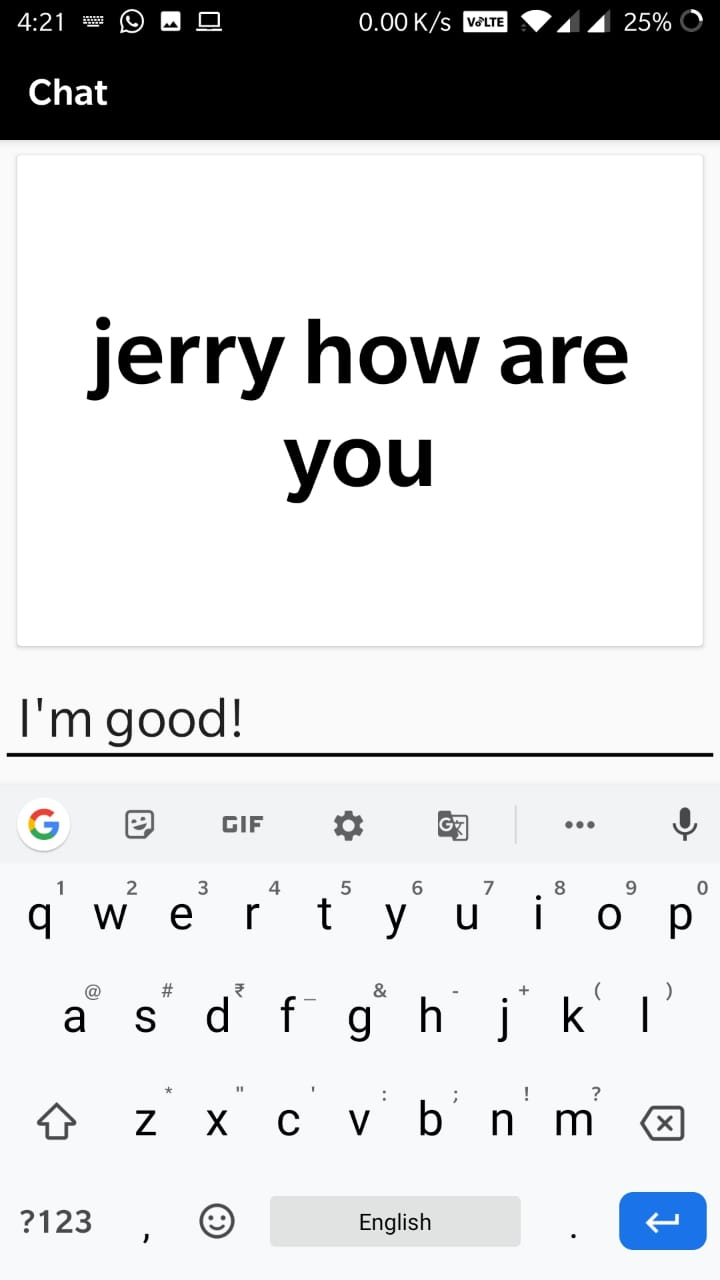
\includegraphics[width=5cm]{TextInput.jpeg} }}%
							\qquad
							\subfloat[Speech]{{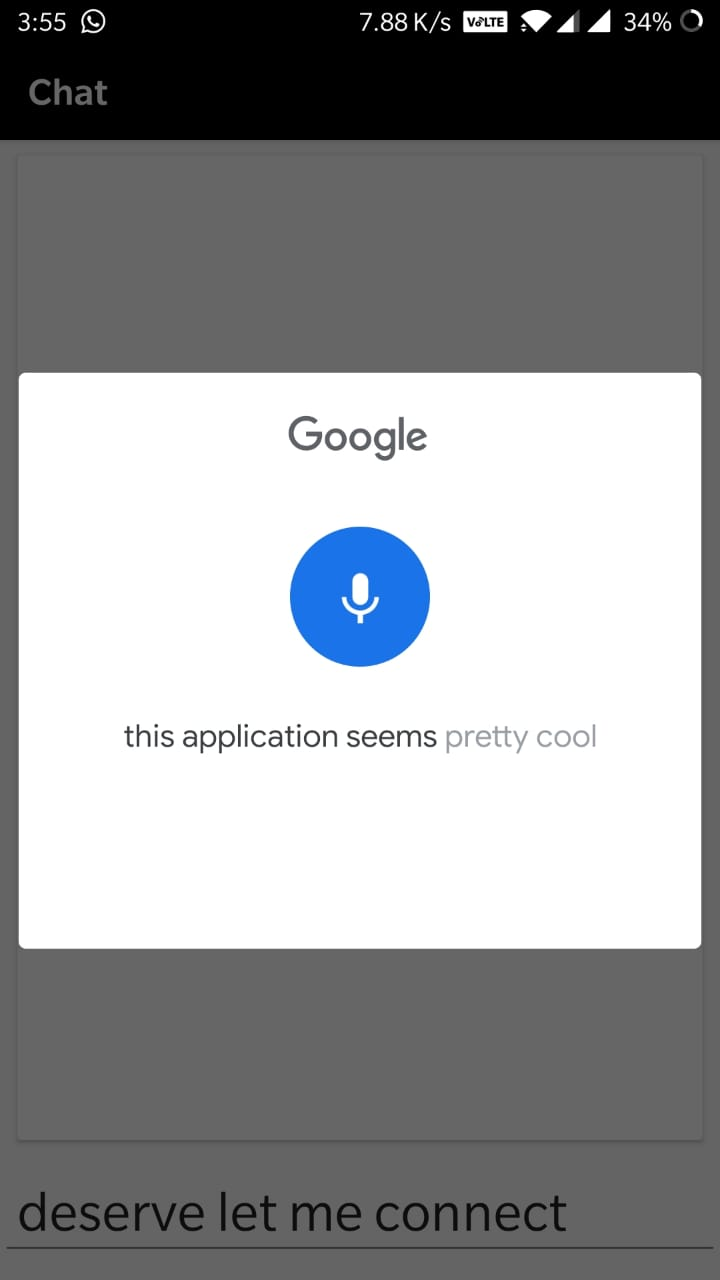
\includegraphics[width=5cm]{SpeechInput.jpeg} }}%
							\caption{Application Input Methods - I}%
							\label{fig:input1}%
						\end{figure}
						\begin{figure}[h]
							\centering
							\subfloat[Morse Code]{{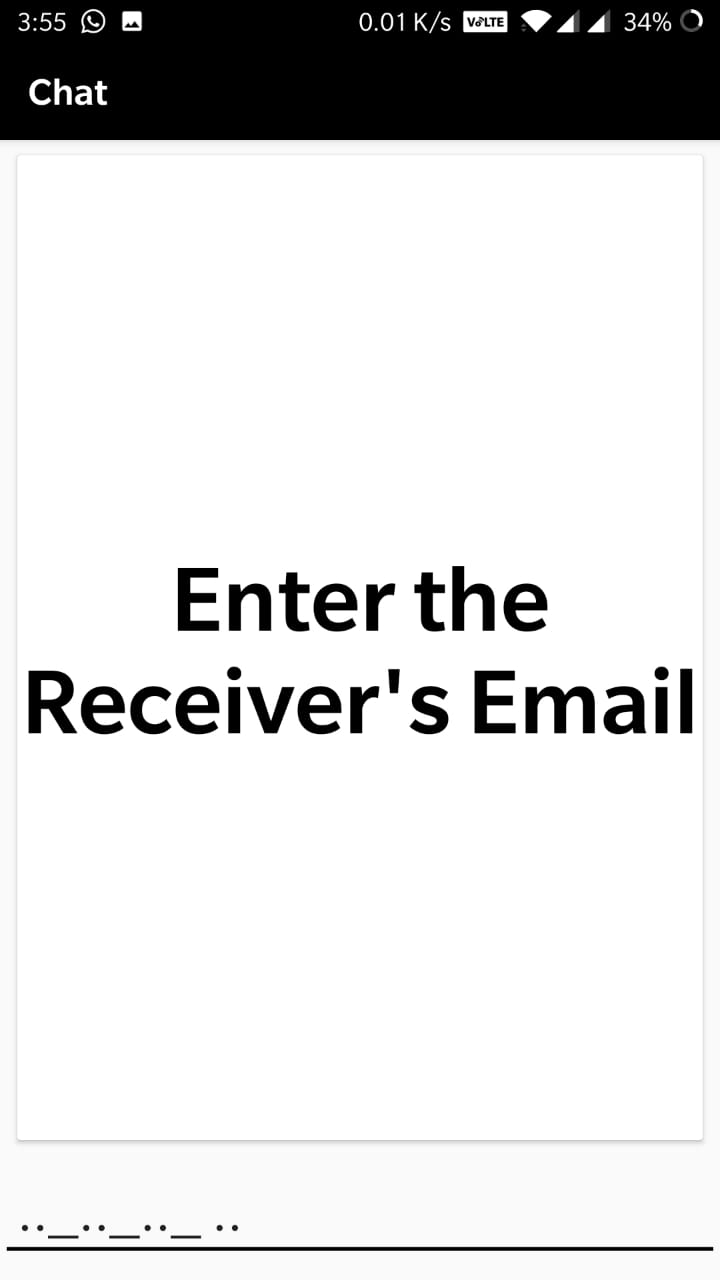
\includegraphics[width=5cm]{MorseInput.jpeg} }}%
							\qquad
							\subfloat[American Sign Language]{{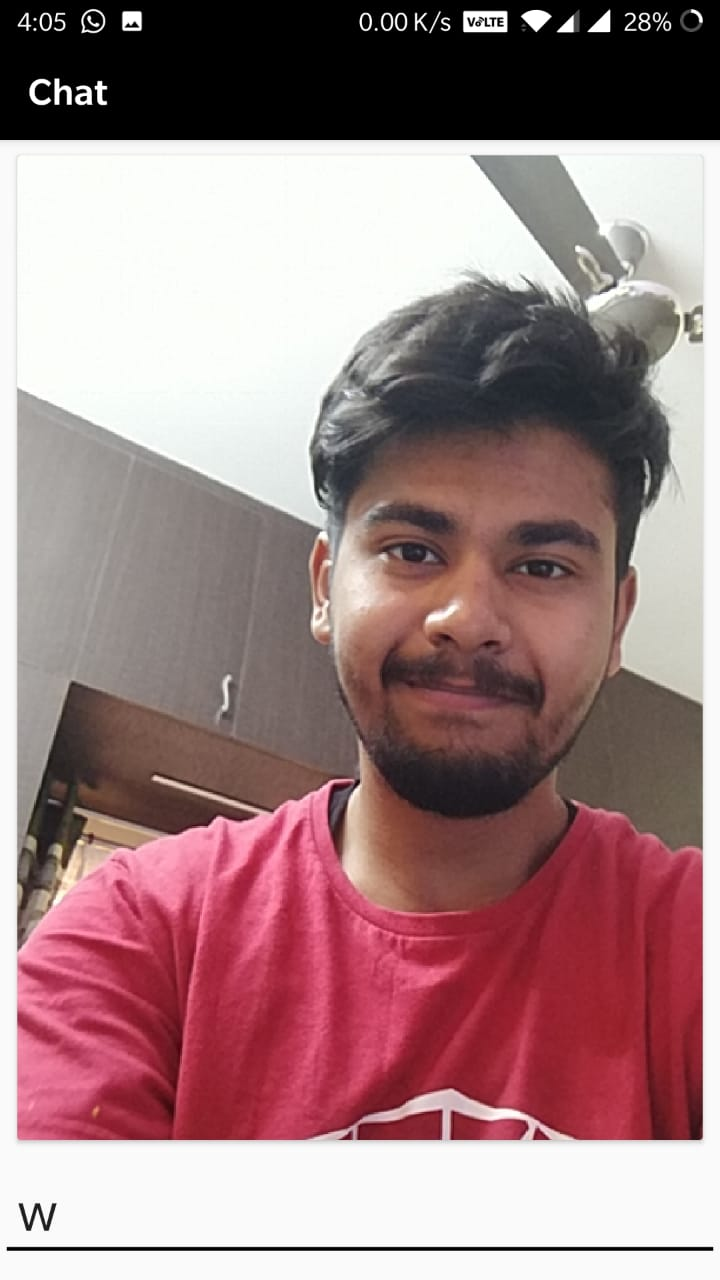
\includegraphics[width=5cm]{ASLInput.jpeg} }}%
							\caption{Application Input Methods - II}%
							\label{fig:input2}%
						\end{figure}
				\subsubsection{The Conversion and Transmission Phase}
						This phase of the application deals with the conversion of the various types of input data (as discussed previously) to a fundamental form, and the transmission of this data from the sender to the receiver.\\

						Here, the fundamental form of data used is the text format which is stored as a String on the database. The tramsmission is acheived with the help of the Firebase APIs that enables us to use Firebase's Realtime Database and Cloud Messaging Services.\\

						The input data, before being sent to the receiver from the sender, is validated and converted to text with the help of certain algorithms designed solely for the purposes of conversion of the input data. Once validated and converted, this text is stored on the Firebase servers as a modified JSON object. This message is then received by the receiver whenever he/she opens the application. Thus, conversion and transmission is achieved in this manner.

				\subsubsection{The Output Phase}
					On similar lines as the input phase, this application uses various forms of output catering to the various categories of the physically-impaired. The various output methods and their use cases are discussed below.
					\begin{itemize}
						\item \textbf{Text - }This form of output can be used by the deaf,  the dumb,  or a combination of both. The tool used for this output method is the default Android text display provided by the Android Operating System.
						\item \textbf{Speech - }This form of output can be used by the deaf, the blind, or a combination of both. The tool used for this output method is the Google Text-to-Speech API which had been discussed in the previous sections.
						\item \textbf{Morse Code - }This form of output can be used by the deaf, the dumb, the blind, or a combination of these. The tool used for this is the Android haptic feedback feature which allows us to set vibration durations of the phone depending on whether the input to the feedback generator is a dot or a dash.
					\end{itemize}	

					One point to note is that the input and output preferences can be set through the `Preferences Page' as shown in Figure~\ref{fig:PrefPage}.\\
					\begin{figure}[h]
						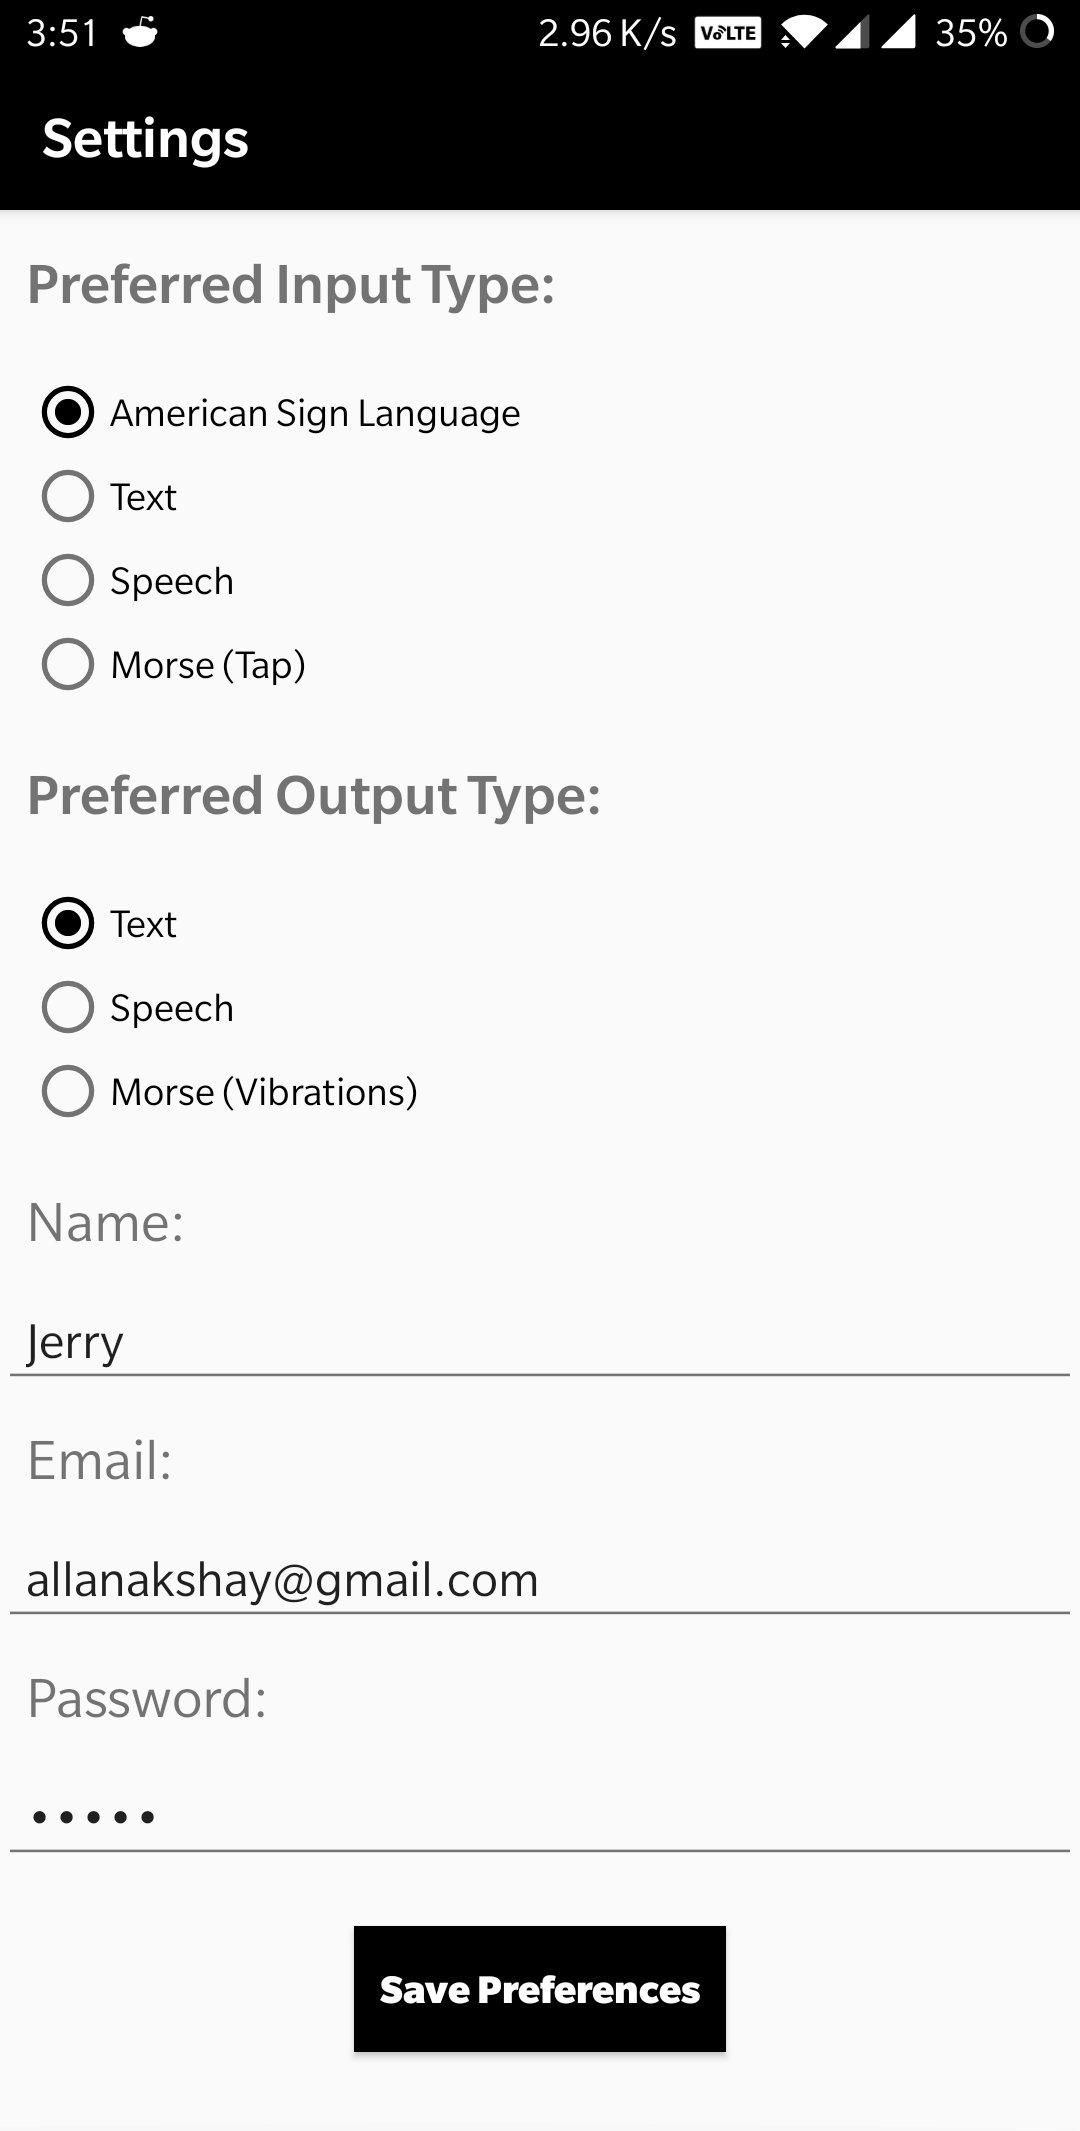
\includegraphics[width=6.5cm]{PrefPage.jpeg}
						\centering
						\caption{Preferences Page}
						\label{fig:PrefPage}
					\end{figure} 

					One can also change their Display Names through the `Preferences Page'. They also have the choice of logging in to a different account through this page.
			\subsection{Database Structure}
				The database of any application plays a crucial role as it stores all the data that is being transacted online through the application. This particular application - Universal Interpreter - uses Firebase as the Database Server.\\

				Firebase is a NoSQL Database Server that stores data as JSON objects instead of tables. The structure of the JSON object for this particular application is shown in Figure~\ref{fig:DataStruct}. The description of this structure is provided in the subsequent sub-sections.\\
				\begin{figure}[H]
					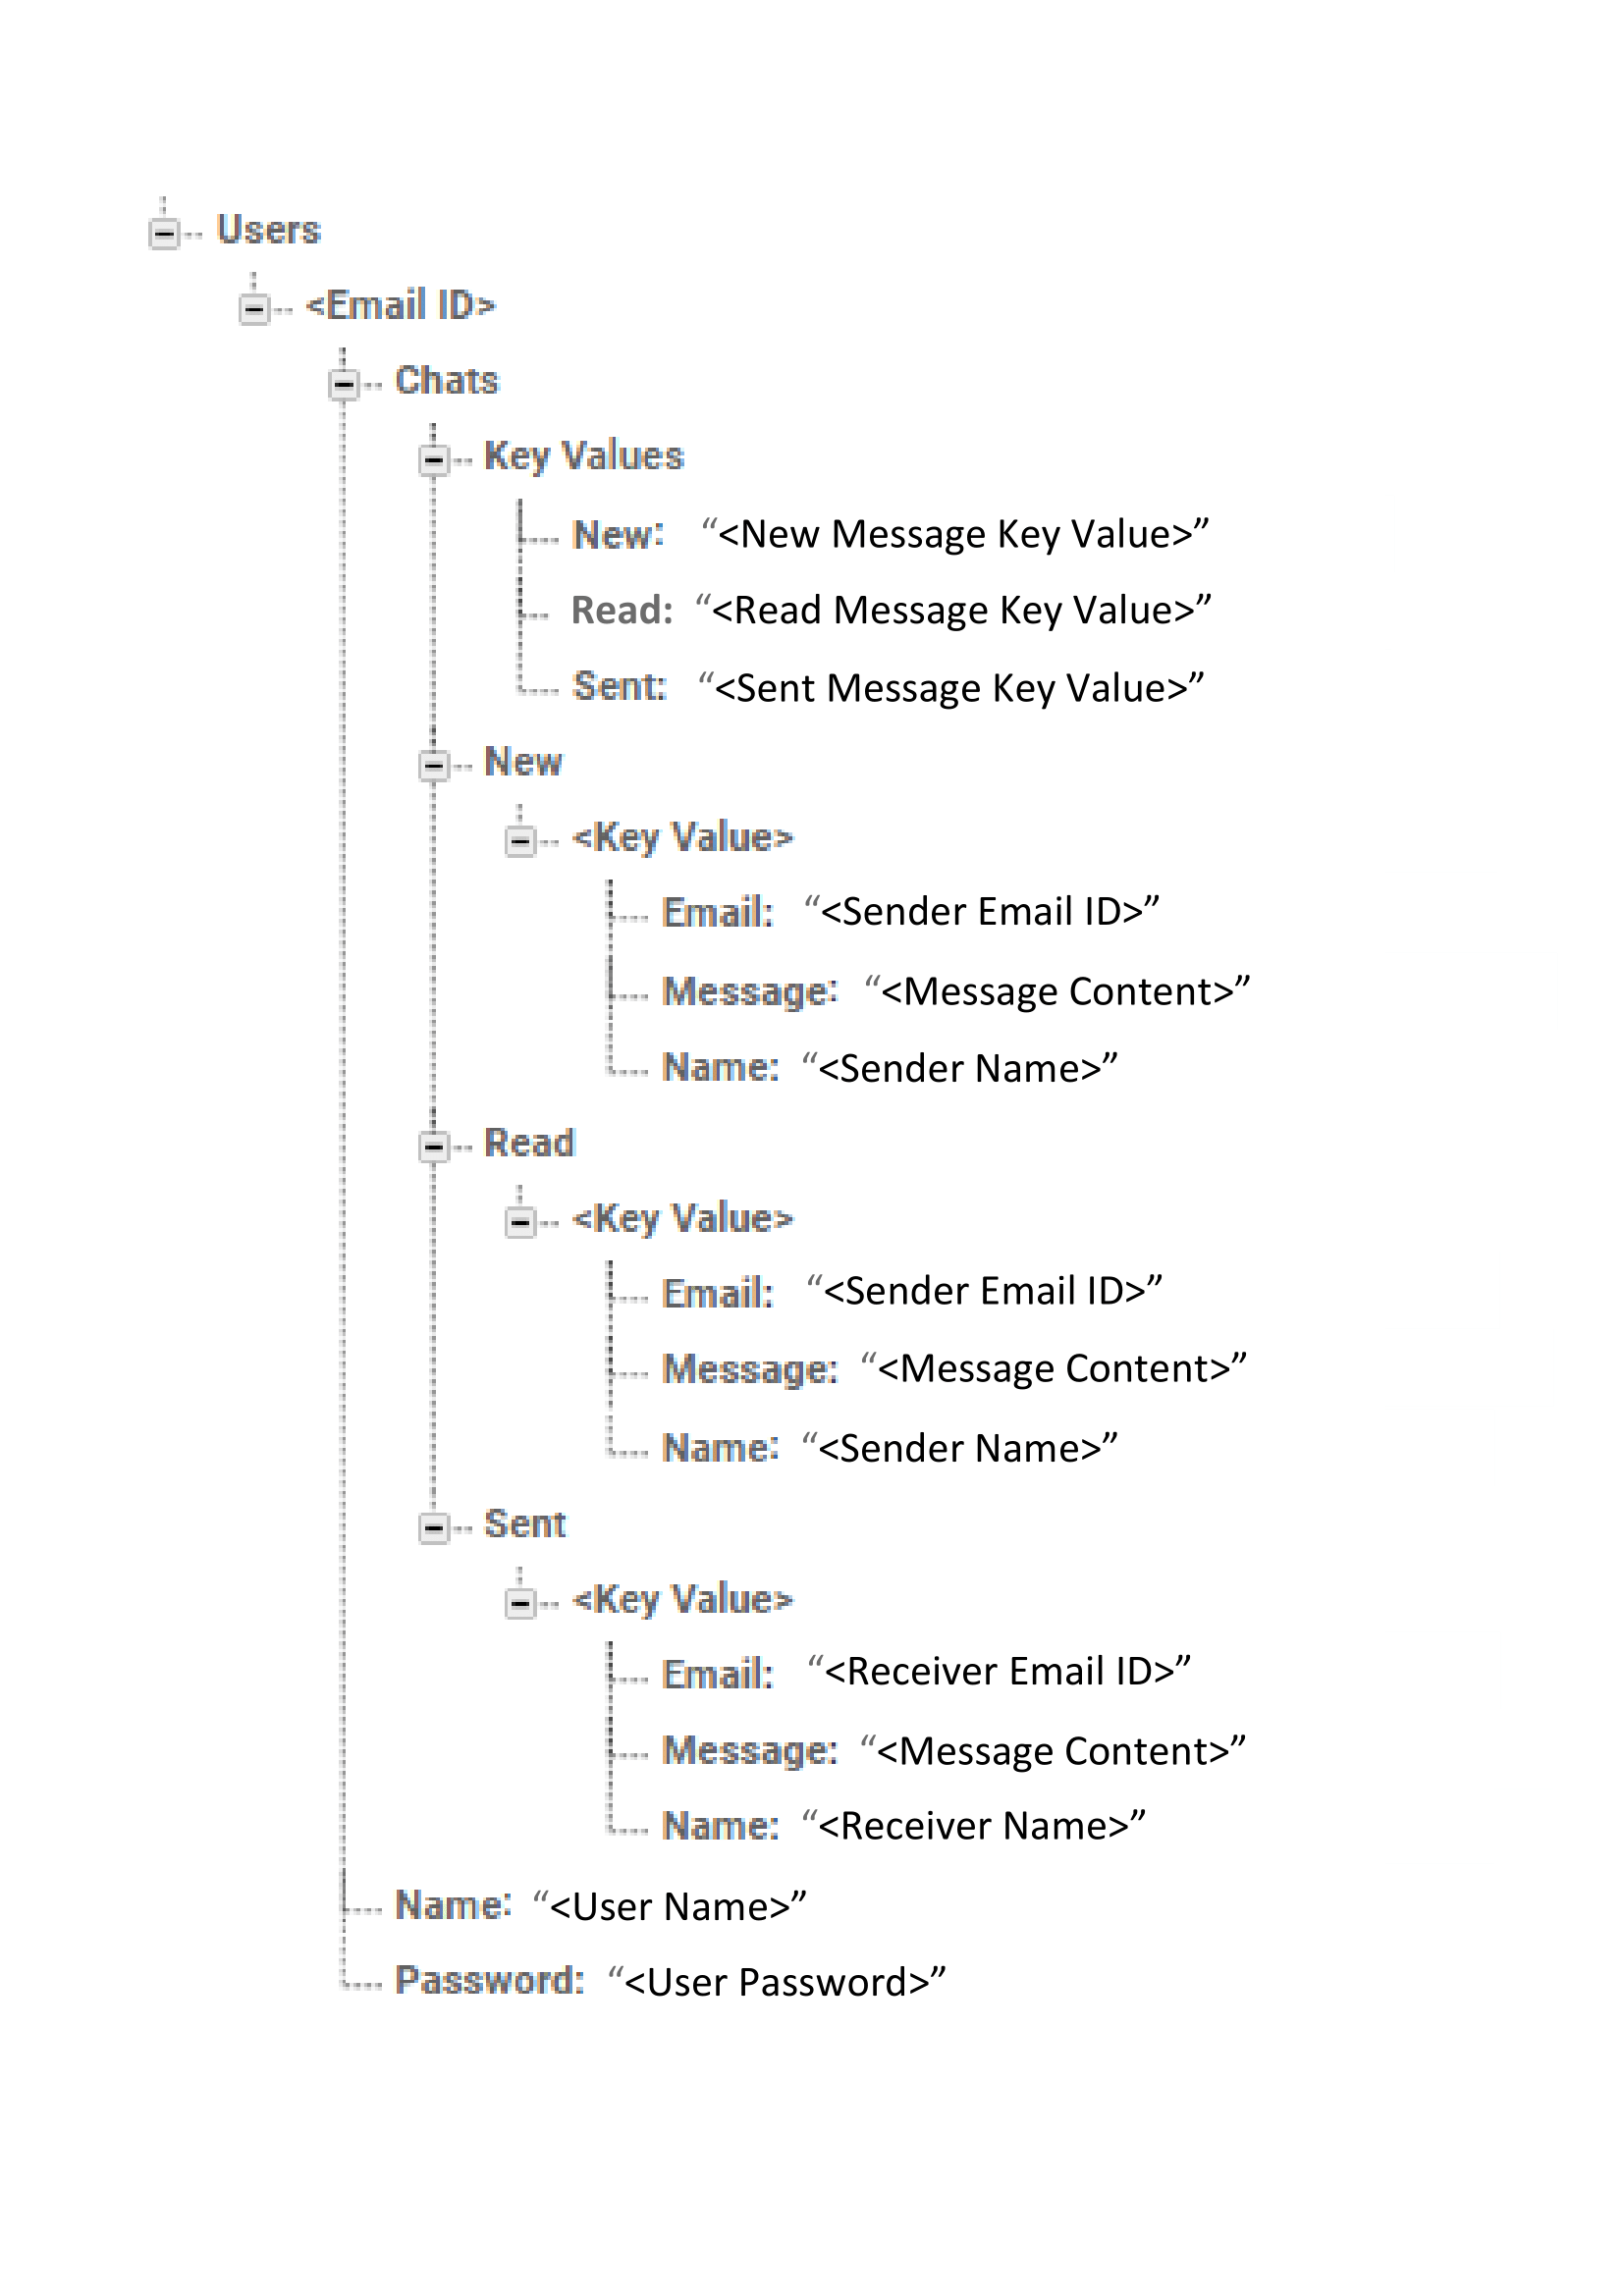
\includegraphics[width=15cm]{DataStruct.png}
					\centering
					\caption{Database Structure}
					\label{fig:DataStruct}
				\end{figure} 
				\subsubsection{The `Users' Block}
					The `Users' block stores the Email-IDs of all the users of the application. Any login to the application will traverse this list to find the respective email id. If the email id doesn't exist, it implies that the user hasn't created an account on the application yet, following which a new account is automatically on the server on behalf of the user.\\

					One more use case where this block is used is when a user needs to send a message to a user he/she has never previously communicated with. The sender will have to enter the `Receiver's Email ID' in the app, and only if the email id exists in the `Users' Block will the sender be allowed to send a message to the desired user. Otherwise, an error message is displayed stating that the user does not exist. This page is depicted in Figure~\ref{fig:ReceivePage}.
					\begin{figure}[h]
						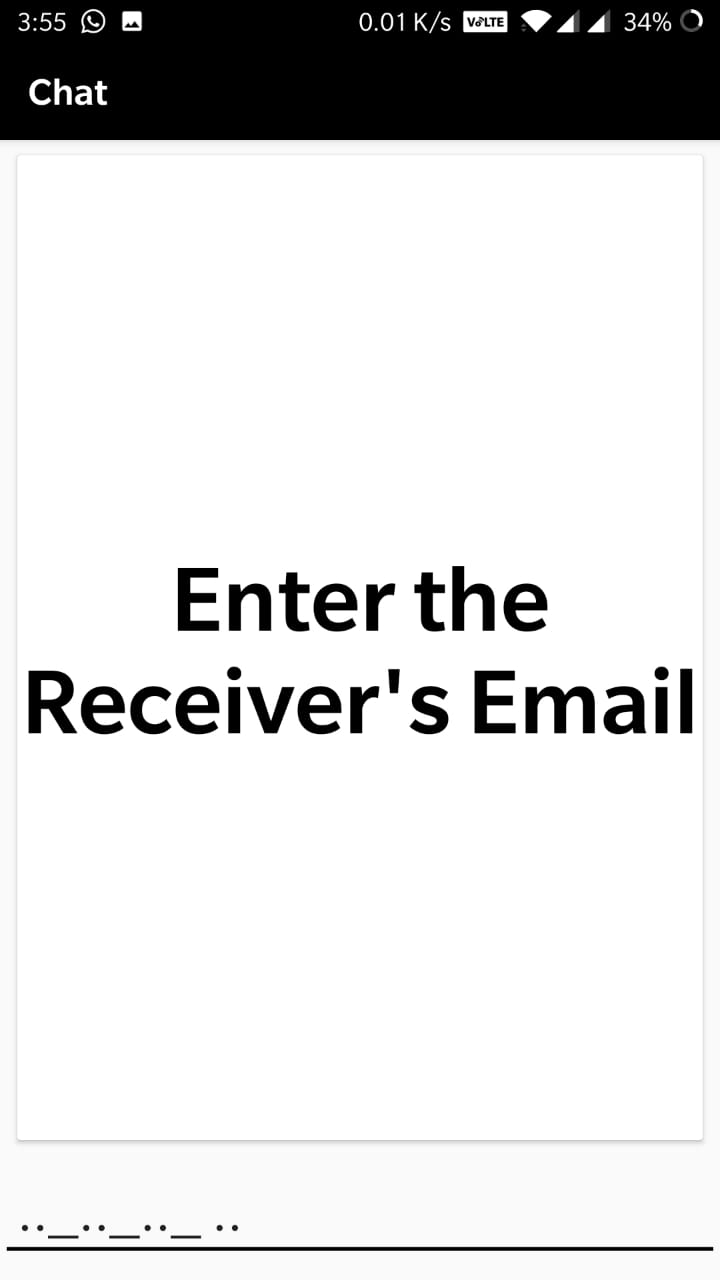
\includegraphics[width=6cm]{ReceivePage.jpeg}
						\centering
						\caption{Communication with a New User}
						\label{fig:ReceivePage}
					\end{figure} 
				\subsubsection{The `Email ID' Block}
					The `Email ID' block stores the Chats for the respective user. This block is particularly used whenever a user opens the app. The app connects to the database and references to the logged in user's email id (present in the `Users' block). Upon referencing, the app uses the `Chats' block to populate the app with the different types of messages - New and Read. The Sent messages exist only as a form of backtracking on the server, in case of breaches or other security concerns.\\

					The `Email ID' block also stores the name of the user and his/her respective password. The 'Name' field is used to store the Display Name of the user and it is the name displayed on the receiver's phone, should a sender send a message across.
				\subsubsection{The `Chats' Block}
					The `Chats' block is used to store the different types of messages - namely the New, Read and Sent messages - of the respective user.\\

					This block makes use of a special sub-block named `Key Values'. This sub-block is used to store the latest message reference keys of the `New', `Read' and `Sent' blocks. This particularly helps to reduce the table lookup time whenever a new message entry is made on the database. 
				\subsubsection{The `New', `Read' and `Sent' Blocks}
					These blocks are used to store the various messages transacted between the various users of the application. Each message has a unique `Key Value' that is assigned to it with the help of the `Key Values' block as discussed in the previous sub-section.\\

					Each message block contains the following fields - Email, Message and Name. The Email field stores the email id of either the sender (in the New / Read block) or the receiver (in the Sent block). Similarly, the Name field stores either the name of the sender (in the New / Read block) or the name of the receiver (in the Sent block). The Message field stores the message content that is transmitted from the sender to the receiver, in the form of text (String).  
		\section{Inception v3 Neural Network}
					As discussed previously, we have used the Inception v3 Neural Network for the purposes of Image Recognition. For our particular application, we have used the model to recognize the hand symbols pertaining to the American Sign Language.\\

					The usage of any Neural Network for any applications depends on the coverage and the efficiency of the following steps - Data Collection, Model Training and Model Predictions. Each of these steps is discussed in detail below.
			\subsection{Data Collection}
					Data Collection involves the collection of data required for training and testing of the Neural Network Model. A data set is a collection of data. In other words, a data set corresponds to the contents of a single database table, or a single statistical data matrix, where every column of the table represents a particular variable, and each row corresponds to a given member of the data set in question.\\

					In Machine Learning projects, we need a training data set. It is the actual data set used to train the model for performing various actions.

					\subsubsection{Need for a Data Set}
						Machine Learning depends heavily on data. Without data, it is impossible for an any Neural Network to `learn'. It is the most crucial aspect that makes algorithm training possible. No matter how great the Neural Network model is or the size of your data set; if your data set is not good enough, your entire Neural Network model will fail to predict accurately.\\

						During any Neural Network development, we always rely on data. From training, tuning, model selection, to testing, we use three different data sets - the training set, the validation set, and the testing set. The validation sets are used to select and tune the final Neural Network Model.\\
						\begin{enumerate}
							\item \textbf{Training Data Set - }The training data set is the set that is used to train an algorithm to understand how to apply concepts such as neural networks, to learn and produce results. It includes both input data and the expected output. Training sets make up the majority of the total data, around 60\%. In testing, the models are fit to parameters in a process that is known as adjusting weights.
							\item \textbf{Testing Date Set -}The testing data set is used to evaluate how well your algorithm was trained with the training data set. In any AI project, we cannot use the training data set in the testing stage because the algorithm will already know the expected output, which is not our goal. Testing sets represent 20\% of the data. The test set is ensured to be the input data grouped together with verified correct outputs, generally by human verification.
						\end{enumerate}

						Figure~\ref{fig:DataCollection} depicts the various data sets and their use cases.
						\begin{figure}[h]
							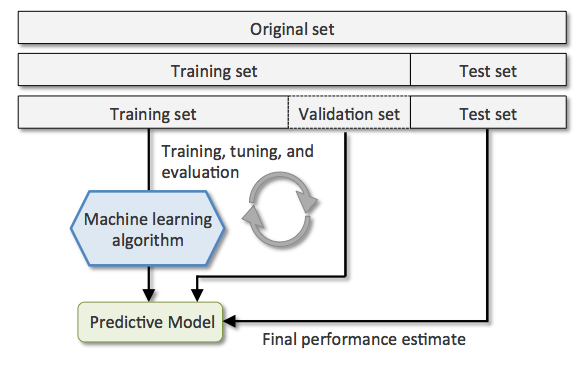
\includegraphics[width=\textwidth]{DataCollection.png}
							\centering
							\caption{Data Sets for a Neural Network Model}
							\label{fig:DataCollection}
						\end{figure}

						For this particular project, our data sets included the hand gestures for all the 26 alphabets of the english language, under different lighting and background conditions. The various hand gestures (or hand symbols) for the American Sign Language are depicted in Figure~\ref{fig:ASLHandSign}.
			\subsection{Model Training}
						Usually, machine learning models require a lot of data in order for them to perform well. Usually, when training a machine learning model, one needs to collect a large, representative sample of data from a training set. Data from the training set can be as varied as a corpus of text, a collection of images, and data collected from individual users of a service. Overfitting is something to watch out for when training a machine learning model.\\

						The Inception v3 Model is a pre-trained model provided by TensorFlow. For the purposes of this application, we apply Transfer Learning to this existing model and re-train it to classify a new set of images (which in our case are the ASL hand symbols).\\

						Using the training data set that we've collected, we train the Neural Network Model using a Python script. Once this training process has completed, we get an updated weights file that help us to perform image recognition operations on any camera image data stream.
						
			\subsection{Model Predictions}
				Predictive modeling uses statistics to predict outcomes. Most often the event one wants to predict is in the future, but predictive modelling can be applied to any type of unknown event, regardless of when it occurred. For example, predictive models are often used to detect crimes and identify suspects, after the crime has taken place.\\

				In many cases the model is chosen on the basis of detection theory to try to guess the probability of an outcome given a set amount of input data, for example given an email determining how likely that it is spam.\\
				\begin{figure}[h]
					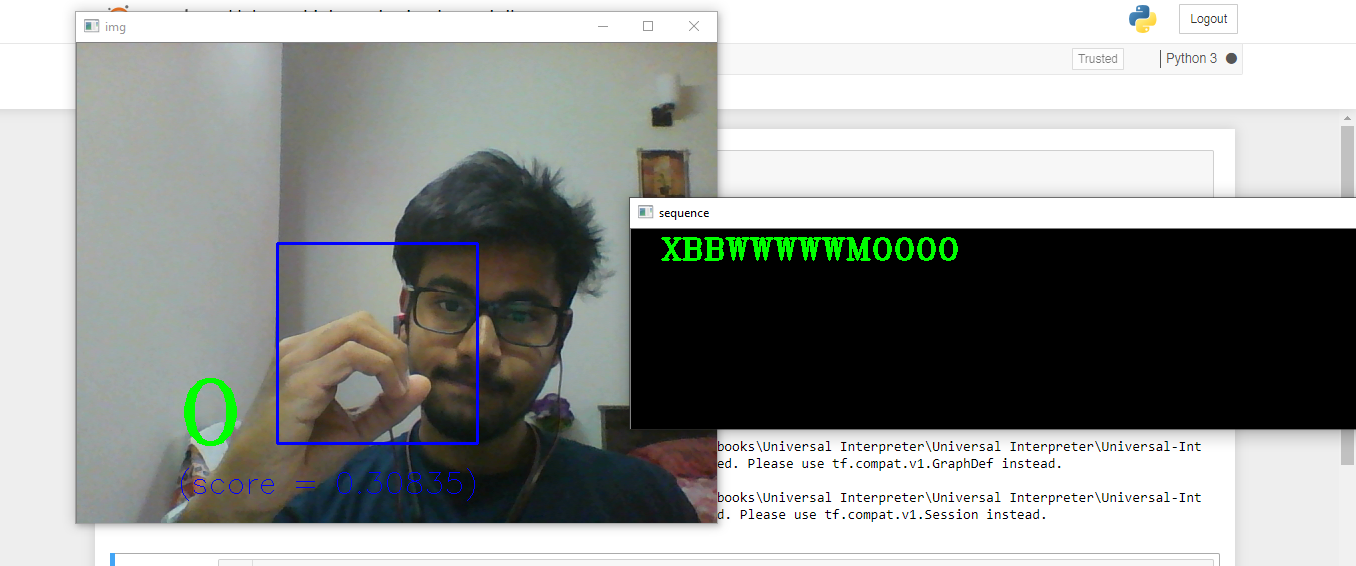
\includegraphics[width=\textwidth]{ModelPred.PNG}
					\centering
					\caption{Prediction with the Inception v3 Model}
					\label{fig:ModelPred}
				\end{figure}

				Models can use one or more classifiers in trying to determine the probability of a set of data belonging to another set. For example, a model might be used to determine whether an email is spam or "ham" (non-spam).\\

				Depending on definitional boundaries, predictive modelling is synonymous with, or largely overlapping with, the field of machine learning, as it is more commonly referred to in academic or research and development contexts. When deployed commercially, predictive modelling is often referred to as predictive analytics.\\

				Predictive modelling is often contrasted with causal modelling/analysis. In the former, one may be entirely satisfied to make use of indicators of, or proxies for, the outcome of interest. In the latter, one seeks to determine true cause-and-effect relationships. This distinction has given rise to a burgeoning literature in the fields of research methods and statistics and to the common statement that "correlation does not imply causation".\\

				In our application, the Inception v3 Model predictions have attained a certain level of predicton accuracy, which can be better improved with the help of a larger training data set with wider coverage in different physical conditions. A sample of the Model Predictions attained in our project are shown in Figure~\ref{fig:ModelPred}.
	\newpage

	%Conclusion

	\chapter{Conclusion}\label{chapter6}
		
	\lhead{\titleref{chapter6}}
				This project has surely been a learning experience for all of us. The exposure we've received to Neural Network Models and the use of these models in real life applications is truly tremendous. The ability to help the physically-impaired with the help of the current technology is surely an eye-opener.\\

				This project, while it remains for now a basic communication application, can be extended for use in various other applications. The very same tools used in this project can be used to provide authentication services to the physically-impaired in banking application scenarios. They can also be used to perform real-time translation of data at public venues such as shopping malls or parks.\\

				We really hope this project of ours could help the needy and make the dominating technologies more accessible to them. We hope this project could help bridge the existent wide gap between the prevalent technological devices and the physically-impaired.

	\newpage

	%References
		
	\lhead{Reference}
	\renewcommand{\bibname}{References}
	\begin{thebibliography}{9}
		\bibitem{latexcompanion} 
		Peter Norvig and Stuart J. Russell.
		\textit{Artificial Intelligence: A Modern Approach}. 
		Prentice Hall, 1994.
	
		\bibitem{latexcompanion} 
		Tom Mitchell.
		\textit{Machine Learning}. 
		McGraw Hill, 1997.

		\bibitem{latexcompanion} 
		Ted Hagos.
		\textit{Android Studio IDE Quick Reference: A Pocket Guide to Android Studio Development}. 
		Apress, 2019.

		\bibitem{latexcompanion} 
		Adam Gerber, Clifton Craig and David Selvaraj.
		\textit{Learn Android Studio: Build Android Apps Quickly and Effectively}. 
		Apress, 2018.

		\bibitem{latexcompanion} 
		Sam Abrahams, Danijar Hafner, Erik Erwitt and Ariel Scarpinelli.
		\textit{TensorFlow For Machine Intelligence: A hands-on introduction to learning algorithms}. 
		Bleeding Edge Press, 2016.

		\bibitem{latexcompanion} 
		Mark Lutz.
		\textit{Learning Python: Powerful Object-Oriented Programming}. 
		O'Reilly Media, 2013.

		\bibitem{latexcompanion} 
		Aur\'elien G\'eron.
		\textit{Hands-On Machine Learning with Scikit-Learn, Keras, and TensorFlow: Concepts, Tools, and Techniques to Build Intelligent Systems}. 
		O'Reilly Media, 2019.

		\bibitem{latexcompanion} 
		Herbert Schildt.
		\textit{Java: The Complete Reference}. 
		McGraw-Hill Education, 2018.

		\bibitem{latexcompanion} 
		Dr. Y. Daniel Liang.
		\textit{Introduction to Java Programming and Data Structures}. 
		Pearson, 2017.

		\bibitem{latexcompanion} 
		Andreas Müller.
		\textit{Introduction to Java Programming and Data Structures}. 
		O'Reilly Media, 2016.


	\end{thebibliography}

	\newpage


\end{document} %Document Ends